\chapter{A Quick Overview of Other Tools}




%-------------------------------------------------------------------
%-------------------------------------------------------------------
%-------------------------------------------------------------------

\section{Developing raw and jpeg Images with Devlop}


%-------------------------------------------------------------------
%-------------------------------------------------------------------
%-------------------------------------------------------------------

\section{Making Ortho Mosaic with Porto}
\label{Porto}

\subsection{Introduction}

{\tt Porto}  is a tool for generating a complete mosaic from a set of \UNCLEAR{single}
ortho images generated by {\tt MicMac}. It is in a very basic state,
a lot of improvement would be required. By the way, I think  it can
still be useful for several applications.

To generate the tool:

\begin{center}
     make -f MakeOrtho
\end{center}

{\tt Porto} expects a parameter file like {\tt MicMac} and {\tt Apero}. It
must contain a structure {\tt CreateOrtho} as specified in {\tt SuperposImage.xml}.

The {\tt ExempleDoc/Boudha} data set contains an example of usage. Run it
by typing:

\begin{center}
                  bin/Porto ../micmac\_data/ExempleDoc/Boudha/ORTHO/Param-Porto.xml
\end{center}

   % - - - - - - - -  -- -  - - - - - - - -  - - - - - - - - - - - - - - - - - - - - - - - -

\subsection{Input to Porto}

The figure~\ref{Resul:Ortho:MM} presents the output of {\tt MicMac} that is used as
input to {\tt Porto}.
The input to {\tt Porto} consists of:

\begin{itemize}

   \item   a global meta-data  file specifying the geo-referencing of the
           DTM associated to the ortho;

  \item  a set of individual ortho-images;

  \item a set of mask images specifying for each ortho which images are visible;

  \item a set of incidence images, specifying the \UNCLEAR{priority};

  \item  a set of XML meta-data  associated to each image.
\end{itemize}


Figure~\ref{Indiv:Ortho} presents some individual ortho-images computed by MicMac on the
Buddha data set. The figure~\ref{Pb:Indiv:Ortho} presents some details of
the problems of each individual ortho-images. Figure~\ref{Incid:Ortho}
presents the incidence images.






\begin{figure}
\begin{tabular}{||c|c|c||}
   \hline \hline
   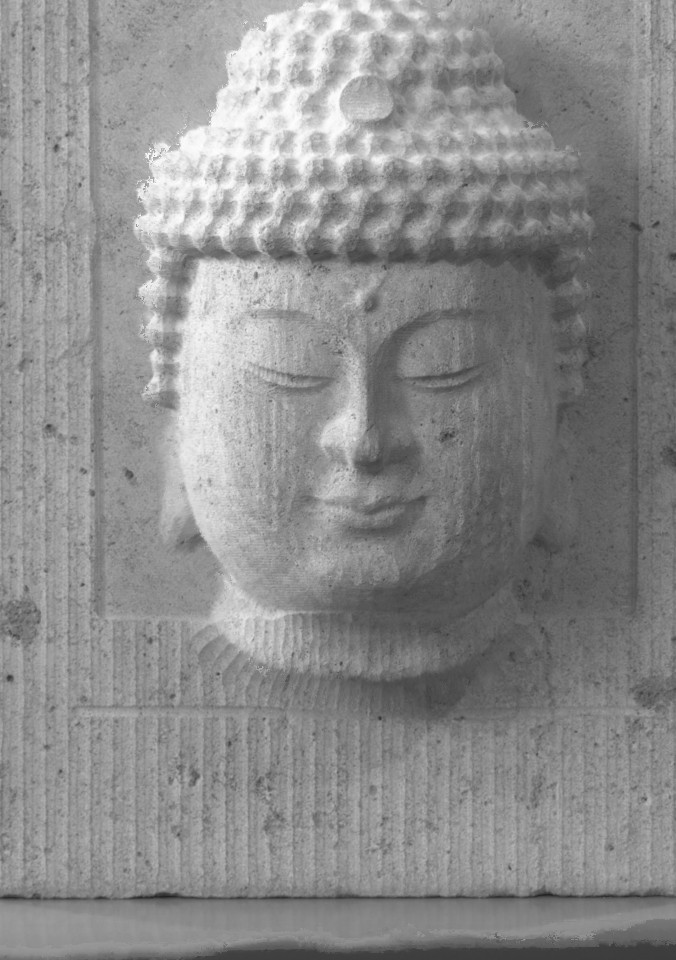
\includegraphics[width=55mm]{FIGS/Boudhas/Ort_IMG_5588.jpg}   &
   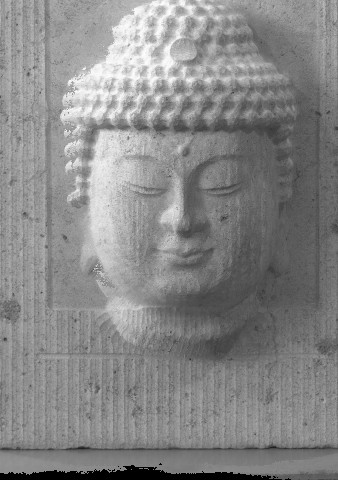
\includegraphics[width=55mm]{FIGS/Boudhas/Ort_IMG_5589.jpg}   &
   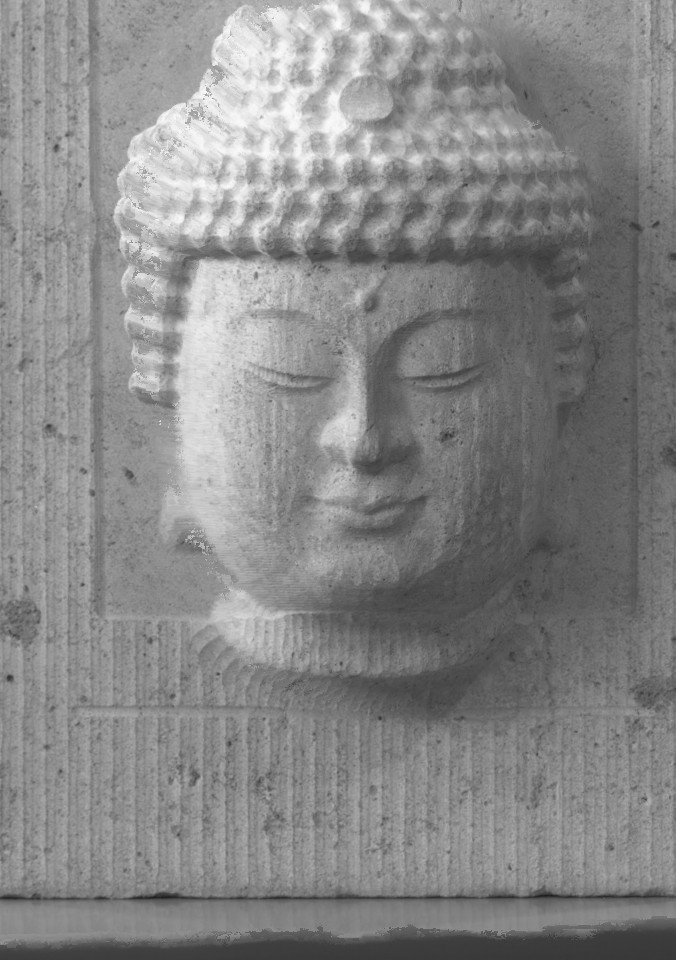
\includegraphics[width=55mm]{FIGS/Boudhas/Ort_IMG_5592.jpg}   \\ \hline  \hline
\end{tabular}
\label{Indiv:Ortho}
\caption{Three of the five individual ortho images}
\end{figure}



\begin{figure}
\begin{tabular}{||c|c||}
   \hline \hline
   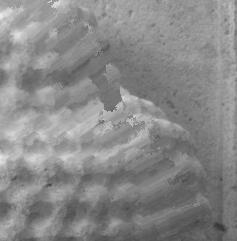
\includegraphics[width=80mm]{FIGS/Boudhas/PB-Ort_IMG_5591.jpg}   &
   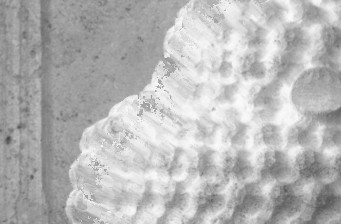
\includegraphics[width=80mm]{FIGS/Boudhas/PB-Ort_IMG_5592.jpg}   \\ \hline  \hline
\end{tabular}
\label{Pb:Indiv:Ortho}
\caption{Zoom on some problems of  individual ortho-image}
\end{figure}



\begin{figure}
\begin{tabular}{||c|c|c|c|c||}
   \hline \hline
   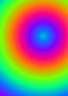
\includegraphics[width=30mm]{FIGS/Boudhas/Incid_IMG_5588_8Bits.jpg} &
   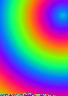
\includegraphics[width=30mm]{FIGS/Boudhas/Incid_IMG_5589_8Bits.jpg} &
   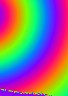
\includegraphics[width=30mm]{FIGS/Boudhas/Incid_IMG_5590_8Bits.jpg} &
   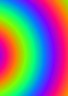
\includegraphics[width=30mm]{FIGS/Boudhas/Incid_IMG_5591_8Bits.jpg} &
   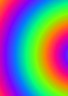
\includegraphics[width=30mm]{FIGS/Boudhas/Incid_IMG_5592_8Bits.jpg} \\ \hline  \hline
\end{tabular}
\label{Incid:Ortho}
\caption{ Incidence images computed for ortho priority}
\end{figure}

In the example {\tt Param-Porto.xml}, the section specifying these inputs is:


{\scriptsize
\begin{verbatim}
    <SectionEntree>
           <FileMNT> ../MEC-7-Ter/Z_Num5_DeZoom1_LeChantier.xml </FileMNT>
           <KeySetIm>  NKS-Set-OfPattern@Ort_(.*)\.tif </KeySetIm>
           <KeyAssocMetaData > NKS-Assoc-ChangPrefixAndExt@Ort_@tif@PC_@xml  </KeyAssocMetaData>
           <KeyAssocNamePC >   NKS-Assoc-ChangPrefixAndExt@Ort_@tif@PC_@tif </KeyAssocNamePC>
           <KeyAssocNameIncH>  NKS-Assoc-ChangPrefixAndExt@Ort_@tif@Incid_@tif </KeyAssocNameIncH>
    </SectionEntree>
\end{verbatim}
}

The {\tt <FileMNT>} is an XML-meta-data file containing information about the DTM produced
by {\tt MicMac}. Its tags have been described in~\ref{Ex:GrTer:RA}. The ortho-mosaic produced
by {\tt Porto} will have the same geo-referencing as the DTM. The other arguments are
keys for describing sets and associations. The functioning is quite classical now:

\begin{itemize}
    \item {\tt <KeySetIm>} describes the set of individual ortho images;
    \item {\tt <KeyAssocMetaData>} is a key for computing the name of XML-Meta data from the name of individual ortho image;
    \item {\tt <KeyAssocNamePC>} is a key for computing the name of the \UNCLEAR{hidden part image} from the name of individual ortho image;
    \item {\tt <KeyAssocNameIncH>} is a key for computing the name of the incidence image from the name of individual ortho image;

    \item \UNCLEAR{this is the same key}, that is used with different parameters; this key allows to change the
          beginning (prefix) of a name and its extension.

\end{itemize}

Here is {\tt PC\_IMG\_5588.xml}, an example of one of the meta-data file:


{\scriptsize
\begin{verbatim}
<MetaDataPartiesCachees>
     <Done>true</Done>
     <Offset>0 0</Offset>
     <Sz>676 960</Sz>
     <Pas>1</Pas>
     <SeuilUse>3</SeuilUse>
     <SsResolIncH>10</SsResolIncH>
</MetaDataPartiesCachees>
\end{verbatim}
}

The important tags are:

\begin{itemize}
   \item {\tt <Offset>} and {\tt <Sz>} specify the position of the individual ortho-photo
         on the DTM. Because, of course, in real example, the individual ortho-photo  will be much smaller
         than the DTM or resulting mosaic, so it will be stored only a sub-rectangle of the global DTM;

   \item {\tt <SeuilUse>} is a real value, use \UNCLEAR{to threshold} the  images ({\tt PC\_IMG\_5588.tif} \dots) and
         defining which pixel must be used;

   \item {\tt <SsResolIncH>} is the resolution of incidence images ({\tt Incid\_IMG\_5588.tif} \dots)
         in fact as these images are very regular, it would be useless to store them at full resolution.

\end{itemize}


As this file have been generated automatically by {\tt MicMac}, in most cases you will
not need to modify it, but it is still good to understand a bit how things work,
in case of problems \dots


   % - - - - - - - -  -- -  - - - - - - - -  - - - - - - - - - - - - - - - - - - - - - - - -

\subsection{Output to Porto}

Once  all these inputs are \UNCLEAR{known}, %nom ou adjectif?
the mosaicing
algorithm is quite obvious:

\begin{itemize}
     \item for each pixel of  the output image:
     \begin{itemize}
          \item select the unmasked image having the lowest incidence.
     \end{itemize}
\end{itemize}

The parameters specifying the output are:

{\scriptsize
\begin{verbatim}
     <SectionSorties>
           <SzDalle>    1000            </SzDalle>
           <SzBrd>      100             </SzBrd>
           <NameOrtho>  Ortho-NonEg-Test-Redr.tif </NameOrtho>
           <NameLabels>  Label-Test-Redr.tif</NameLabels>
     </SectionSorties>
\end{verbatim}
}

{\tt NameOrtho} specifies the name of the ortho mosaic. {\tt NameLabels} is an optional
argument, when specified, {\tt Porto} creates a label image indicating for each pixel which
individual  image is to be used for \UNCLEAR{filling the geometry}.  \UNCLEAR{Figure~\ref{Resul:Ortho}} %pas bon le nr de la fig
presents the main results.


\begin{figure}
\begin{tabular}{||c|c||}
   \hline \hline
   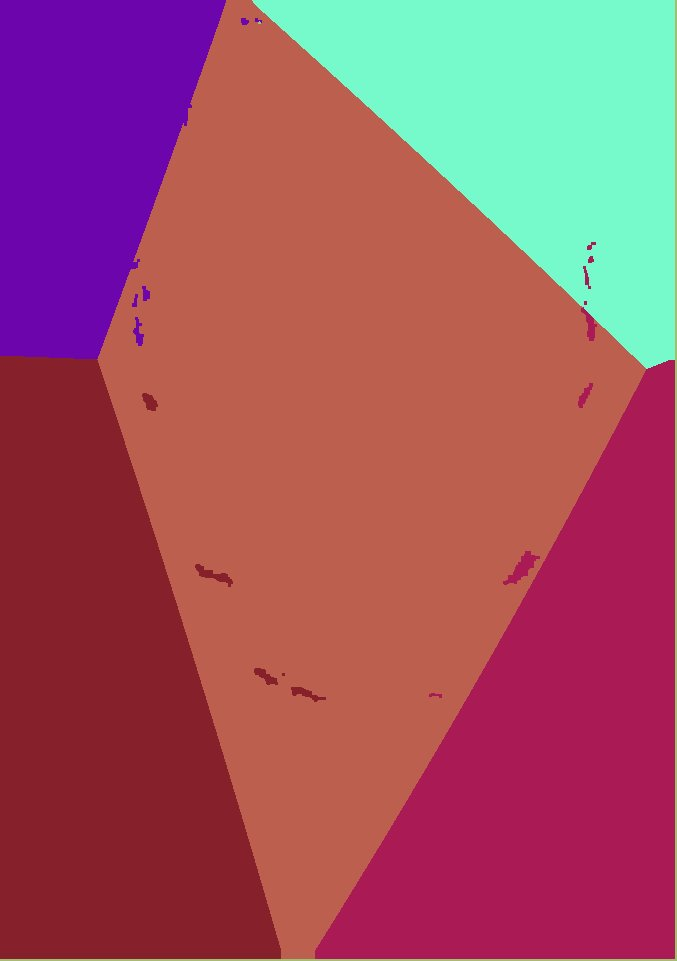
\includegraphics[width=80mm]{FIGS/Boudhas/Label-Test-Redr.jpg}   &
   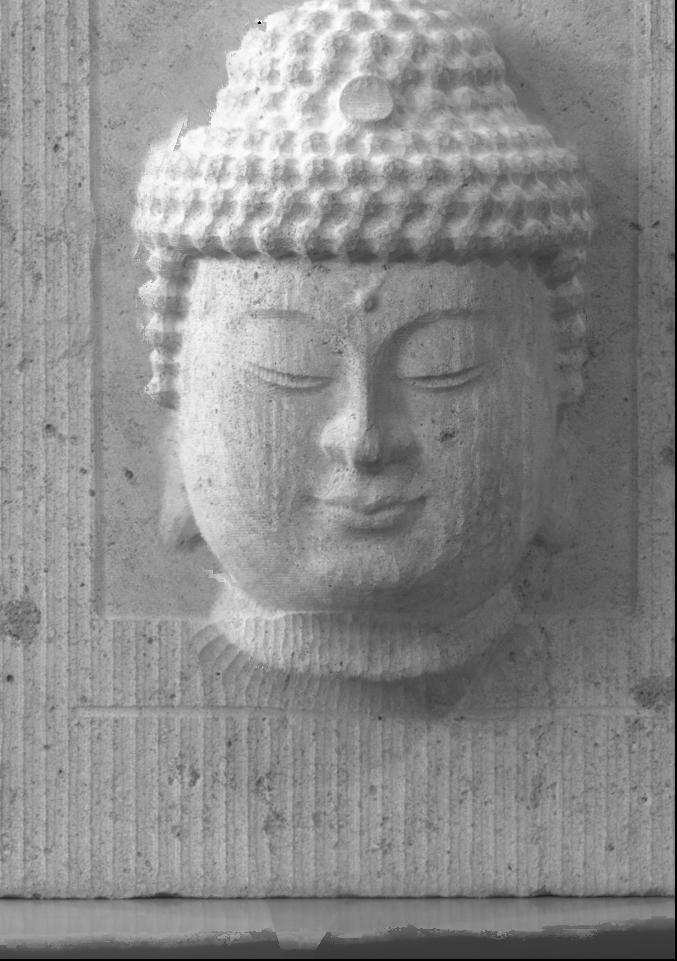
\includegraphics[width=80mm]{FIGS/Boudhas/Ortho-NonEg-Test-Redr.jpg}   \\ \hline  \hline
\end{tabular}
\label{Resul:Ortho}
\caption{Computed label images and resulting ortho images}
\end{figure}



   % - - - - - - - -  -- -  - - - - - - - -  - - - - - - - - - - - - - - - - - - - - - - - -
   % - - - - - - - -  -- -  - - - - - - - -  - - - - - - - - - - - - - - - - - - - - - - - -
   % - - - - - - - -  -- -  - - - - - - - -  - - - - - - - - - - - - - - - - - - - - - - - -

\section{V.O.D.K.A.}
\label{V.O.D.K.A.}

\subsection{Theory}

The vignetting is an optical effect that results in a gradual radial drop-off in images (the corners of images are relatively darker than the center). The figure (\ref{image_vignette}) shows an example of this effect.

\begin{figure}[htb]
\centering
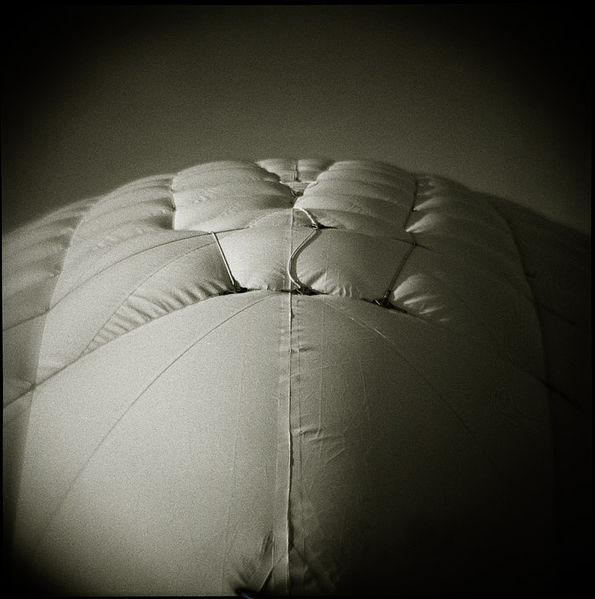
\includegraphics[width=6cm]{FIGS/Arsenic/595px-Swanson_tennis_center.jpg}
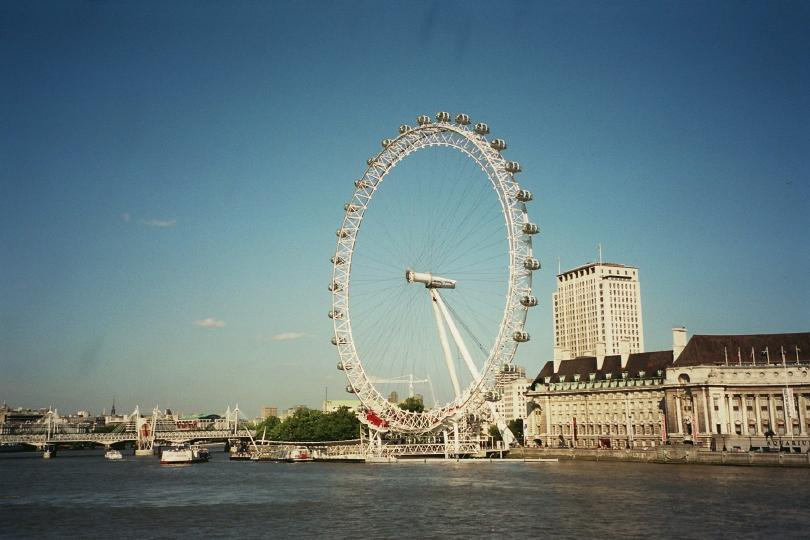
\includegraphics[width=6cm]{FIGS/Arsenic/London_eye_501588_fh000038.jpg}
\caption{
Different vignetting effect
%Vignette from the Nikkor 18-105 mm VR, F/3.6,18mm, fixed on a Nikon D90. The image is one of an homogeneous grey field
}
\label{image_vignette}
\end{figure}

Read more about vignetting :
\begin{itemize}
   \item \url{http://en.wikipedia.org/wiki/Vignetting}
   \item \url{http://fr.wikipedia.org/wiki/Vignettage}
\end{itemize}

\subsection{Name and function}
Vodka stands for "\textit{Vignette Of Digital Kamera Analysis}".

This command estimates the vignetting effect for a set of images with the same aperture and focal length without the need of a laboratory setup (classically an integrating sphere). The vignette model that is used is an even 6th degree polynomial function centered on the middle of the image. With r the distance to the center of the image and $\alpha$, $\beta$ and $\gamma$ the polynomial coefficients, we have : \[V(r)=1+ \alpha r^2 + \beta r^4 + \gamma r^6\]


The computation of the model uses a RANSAC based algorithm to solve the sets of equation of the following type (where $G_{i}$ is the grey value of a tie point for the image i and r the distance to the center of the image) : \[ G_{1}-G_{2}=\alpha(G_{2}*r_{2}^2-G_{1}*r_{1}^2)+\beta(G_{2}*r_{2}^4-G_{1}*r_{1}^4)+\gamma(G_{2}*r_{2}^6-G_{1}*r_{1}^6) \]

Between 9 and 30 points are randomly selected from the tie points and a solution is computed using least square matching. The solution is then awarded a score : \[Score=\frac{P_{inliers}}{EMP}\].

Where:
\begin{itemize}
\item \textit{$P_{inliers}$} the percentage of the tie points complying with the model ($\pm 2\%$) $\Rightarrow$ for good models, a value about 20\% to 40\% is expected.

\item \textit{EMP} the mean error between the model and the points weighted by $min(r_{1},r_{2})$ to increase the importance of points away from the image center (and therefor more influenced by vignetting).
\end{itemize}


\subsection{Input data}
To use this command, a set of images with the same aperture and focal length, taken in a stable illumination setting is necessary. The command also requires the computation of tie points (through Tapioca).


Calling the command is done with the following command line (where ImagesPattern is the regular expression describing the set of images ) : \[mm3d\;Vodka\;ImagesPattern\]

Multiple datasets can be processed at once, the program would then sort the images in subsets with the same aperture and focal length and give a solution for each subset.

\subsection{Output data}
For each aperture/focal length combination in the input set, the commands create a floating point .tif file of the image's size named Vignette/Foc0000Dia111.tif, where 0000 is the focal length in millimeters and 111 the aperture times 10.


Corrected images can also be created if asked by the user, mostly for quality checking (see bellow).


\subsection{Options}
\begin{itemize}
\item{\textit{DoCor (bool)} toggle the creation of corrected images (Def=false)}
\item{\textit{InCal (string)} Name of folder with vignette calibration tif file (if previously computed)}
\item{\textit{InTxt (string)} True if homologous points have been exported in txt (Def=false)}
\item{\textit{Out (string)} Output folder (Default=Vignette)}
\end{itemize}

\subsection{How to use VODKA}
Vodka is to be used to compute a vignette calibration. The best results are obtained with images where tie points are at different distances from the image center in the images that generated them, typically non-convergent images.


The output files should then be placed in a folder with other images taken with the same camera and the same aperture/focal length combination. The images that will be created in the Tmp-MM-Dir (and therefor used by every other commands) when the proper VODKA output files are present will be corrected using those files. If you want to use the VODKA results on the images used to compute it, you should place the VODKA output files in the images' directory and delete the Tmp-MM-Dir folder.

   % - - - - - - - -  -- -  - - - - - - - -  - - - - - - - - - - - - - - - - - - - - - - - -
   % - - - - - - - -  -- -  - - - - - - - -  - - - - - - - - - - - - - - - - - - - - - - - -
   % - - - - - - - -  -- -  - - - - - - - -  - - - - - - - - - - - - - - - - - - - - - - - -

\section{Vignetting correction}

\subsection{How MicMac use vignetting ?}

Each time MicMac encouter a Raw or Jpg image, it create a copy in tiff format, only tiff 
copy are really used by MicMac. It can be 
in $16$ bits or $8$ bits, in $1$ or $3$ channel, so several copy may exist in the {\tt Tmp-MM-Dir}
folder. For creating the tiff image, if there exist a vignetting image it is used to divide
the image.

\subsection{Command {\tt StackFlatField}}
\subsection{Command {\tt PolynOfImage}}

   % - - - - - - - -  -- -  - - - - - - - -  - - - - - - - - - - - - - - - - - - - - - - - -
   % - - - - - - - -  -- -  - - - - - - - -  - - - - - - - - - - - - - - - - - - - - - - - -
   % - - - - - - - -  -- -  - - - - - - - -  - - - - - - - - - - - - - - - - - - - - - - - -

\section{A.R.S.E.N.I.C}
\label{A.R.S.E.N.I.C.}
\subsection{Name and function}
ARSENIC stands for \textit{Automated Radiometric Shift Equalization and Normalization for Inter-image Correction}.


This function corrects the key images used for coloring point clouds in order to have a smooth transition between sub-clouds of the same scene. It is designed to be used with the "GeomImage" correlation geometry.


\textcolor{red}{ This function is not designed for the equalization of images prior to image mosaicing}

\subsection{Input data}
\label{inputArsenic}

ARSENIC require a depth map for each image that will be equalized, computed with MICMAC/Malt. The dense radiometric tie point algorithm used in this program requires very well co-registered depth maps (or point clouds).
Calling the command is done with the following command line (where ImagesPattern is the regular expression describing the set of images ) :\[mm3d\;Arsenic\;ImagesPattern\]

\subsection{Output data}
The output of this command is the corrected images, by default in a folder called Arsenic. These images can then be used to color a point cloud through Nuage2Ply.

\subsection{Options}
\begin{itemize}
\item{\textit{TPA (Tie Point Accuracy - int)} defines the precision threshold for the tie points (def=16, means $\frac{1}{16}$ of pixel resolution)}
\item{\textit{ResolModel (int)} defines the resolution of the model to be used in the tie point computation (def=16 for DeZoom 16)}
\item{\textit{InVig (string)} defines a vignette calibration folder (if any)}
\item{\textit{Out (string)} defines the output directory}
\item{\textit{NbIte (string)} defines the number of iterations of the process (def=5)}
\item{\textit{ThreshDisp (string)} defines the disparity threshold between the tie points (Def=1.4 for 40\%)}
\end{itemize}

\subsection{Algorithm}

\subsubsection{Tie point detection}

In order to have a more accurate, denser and more interest-zone focused set of tie points, the tie points are extracted from the result of the dense correlation.


 Every point situated in the mask of a key image is projected in 3D through the depth map generated by MICMAC/Malt, then reprojected in the other key images and finally projected again in 3D if the second projection resulted in a point in the secondary key image's mask. If the two 3D projections result in a similar point (the concept of similarity being defined through the TPA option : the maximum distance between two 3D projections that validates the points being $PixelResolution/TPA$). For each validated point, the image coordinates of the point in the key image is recorded, as well as the factors $K$ between the pixel values of each images for all channels : \[K=(1+G_{j})/2*G_{i}\]
 With \textit{G} a grey value, \textit{i} the primary key image and \textit{j} the secondary image that generated the tie point. A tie point is therefor an object with 5 values, $Point=(X,Y,K_{R},K_{G},K_{B})$. The $+1$ is a call to the initial value.

\subsubsection{Equalization}

In a first step, a correction factor is computed for each tie point with an inverse distance weighting and a self weighting value (the image is self influencing). For each radiometric channel of each point, $j$, we have the following formula ($i$ is the tie point currently used in the interpolation):
\[Cor(TiePointj)=\sum_{i=1}^{n} \frac{(K_{i})/2}{\sqrt{(X_{i}-X_{j})^2+(Y_{i}-Y_{j})^2}}\]

This process is then iterated. A filtering system is yet to be developed to prevent radiometric outliers to push the model after too many iterations. An outlier is a point where Kr, Kg or Kb is more than \textit{ThreshDisp}\% different than the average value for the image considered.


The corrected tie points are then applied to a grid also through inverse distance weighting, the interpolated to the whole image through bilinear interpolation. The grid is computed by the formula bellow, with $i$ the tie point index and $(X,Y)$ the grid point's coordinates : \[Cor(X,Y)=\sum_{i=1}^{n} \frac{K_{i}}{\sqrt{(X_{i}-X)^2+(Y_{i}-Y)^2}}\]

\begin{figure}[H]
\centering
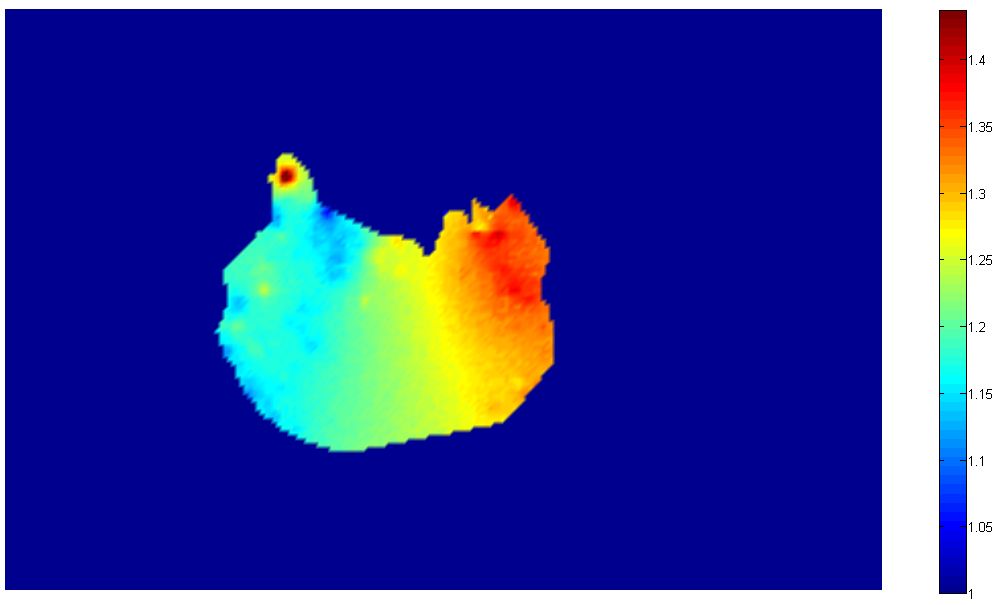
\includegraphics[width=15cm]{FIGS/Arsenic/SurfCorr.png}
\caption{Example of a correction surface}
\label{SurfCorr}
\end{figure}


\subsection{How to use ARSENIC}

Once the appropriate input data (see~\ref{inputArsenic}) is computed, the command can be run. The images produced in the output folder are to be used as "Attr" arguments in the "Nuage2Ply" command to produce equalized sub-point clouds.

%***************************%
\section{Comparaison tools}
This part concerns all the tools to compare files or results of calculations coming from {\tt MicMac}:

%-----------------%
\subsection{CmpOri}
The {\tt CmpOri} command computes average norme differences of all external parametrs of images from 2 Ori-XXX/ folders.

\begin{verbatim}
*****************************
*  Help for Elise Arg main  *
*****************************
Mandatory unnamed args : 
  * string :: {Full Name (Dir+Pattern)}
  * string :: {Orientation 1}
  * string :: {Orientation 2}
Named args : 
  * [Name=DirOri2] string :: {Orientation 2}
  * [Name=XmlG] string :: {Generate Xml}
  * [Name=CSV] string :: {Generate detail CSV (excel compatible) for each image}
  * [Name=Ply] string :: {Generate .ply File}
  * [Name=ColXY] Pt3di :: {color for XY component of .ply}
  * [Name=ColZ] Pt3di :: {color for Z component of .ply}
  * [Name=ColOri] Pt3di :: {color for orientation component of .ply}
  * [Name=ScaleC] REAL :: {Scale for camera center difference, the center diff is displayed when this option is activated}
  * [Name=ScaleO] REAL :: {Scale for camera orientation difference, the ori diff is displayed when this option is activated}
  * [Name=F] REAL :: {approximate value of focal length in (m), Def=0.03875m for Camlight}

\end{verbatim}

Example :
\begin{verbatim}
mm3d CmpOri ".*JPG" Ori-Bascule/ Ori-Compense/ XmlG=Delta_Basc_Comp.xml
\end{verbatim}

For example the result displayed and saved in {\tt Delta\_Basc\_Comp.xml} :
\begin{verbatim}
<?xml version="1.0" ?>
<XmlTNR_TestOriReport>
     <OriName>RTL-Compense-AllPts</OriName>
     <TestOriDiff>false</TestOriDiff>
     <DistCenter>0.0397097570172935677</DistCenter>
     <DistMatrix>3.87112370850761372e-07</DistMatrix>
</XmlTNR_TestOriReport>
\end{verbatim}


%-------------------%
\subsection{CmpCalib}
The {\tt CmpCalib} command compares two files of calibrations Ori-XXX/AutoCal\_Foc-XXX.xml (in general of the same camera).

\begin{verbatim}
mm3d CmpCalib -help
*****************************
*  Help for Elise Arg main  *
*****************************
Mandatory unnamed args : 
  * string :: {First calibration file}
  * string :: {Second calibration file}
Named args : 
  * [Name=Teta01] REAL
  * [Name=Teta02] REAL
  * [Name=Teta12] REAL
  * [Name=L1] INT
  * [Name=SzW] INT
  * [Name=DynV] REAL
  * [Name=Out] string :: {Result (Def=Name1_ecarts.txt)}
  * [Name=DispW] bool :: {Display window}
  * [Name=XmlG] string :: {Generate Xml}
\end{verbatim}

Example :
\begin{verbatim}
mm3d CmpCalib Ori-Basc/AutoCal_Foc-35000_Cam.xml Ori-Comp/AutoCal_Foc-35000_Cam.xml Out=Delta_Calib.txt
\end{verbatim}

Internal parameters of a camera cannot be directly compared. The command estimates a rotation to align the parameters.
The output file {\tt Delta\_Calib.txt} contains a function which gives the differences between the two sets of calibration models as function of the radius and 
a grid which provides planimetric vector deviation between each rays directions. Example of output :

\begin{verbatim}
--------------  Ecart radiaux  -----------
 Rayon   Ecart
 0.000000 0.035861
 200.000000 0.094960
 400.000000 0.184629
 ...
 --------------  Ecart plani  -----------
Im.X Im.Y  PhG.X Phg.Y Ec
5017.600000 3763.200000 -0.855326 -0.588127 1.038015
5017.600000 3394.560000 -0.951363 -0.529560 1.088818
5017.600000 3025.920000 -0.988994 -0.465235 1.092956
...
\end{verbatim}

%----------------%
\subsection{CmpIm}
The {\tt CmpIm} command computes deviations between 2 images.

\begin{verbatim}
mm3d CmpIm -help
*****************************
*  Help for Elise Arg main  *
*****************************
Mandatory unnamed args : 
  * string :: {First image name}
  * string :: {Second image name}
Named args : 
  * [Name=FileDiff] string :: {Difference image output file}
  * [Name=Dyn] REAL :: {Dynamic of difference}
  * [Name=Brd] Pt2di :: {Border to eliminate}
  * [Name=OkSzDif] bool :: {Process files with different sizes}
  * [Name=Mul2] REAL :: {Multiplier of file2 (Def 1.0)}
  * [Name=UseFOM] bool :: {Consider file as DTSM and use XML FileOriMnt}
  * [Name=ColDif] REAL :: {Color file of diff using Red/Blue for sign}
  * [Name=XmlG] string :: {Generate Xml}

\end{verbatim}
%------------------%
\subsection{CompMAF}
The {\tt TestLib CompMAF} command computes differences between 2 image measurement files without the specification on image order.

\begin{verbatim}
mm3d TestLib CompMAF
*****************************
*  Help for Elise Arg main  *
*****************************
Mandatory unnamed args : 
  * string :: {Directory}
  * string :: {Image pattern}
  * string :: {MAF File 1}
  * string :: {MAF File 2}
Named args : 
  * [Name=Out] string :: {Output name of the generated CmpMAF file, Def=CmpMAF.xml}

\end{verbatim}

The difference is computed with reference to the first MAF file. If the measurement of one GCP is measured on the same image for both files, the difference between two measurements is calculated. If not, the value of the first MAF file is conserved.

Example :
\begin{verbatim}
mm3d CompMAF ./ img_029.*.tif MAF1.xml MAF2.xml Out=Comp_MAF1_MAF2.xml
\end{verbatim}

%------------------%
\subsection{CmpTieP}

%--------------------%
\subsection{CmpOrthos}

%---------------------%
\subsection{CmpTrajGps}


%***************************%
\section{Miscellaneous tools}

%------------------------%
\subsection{TestLib PackHomolToPly}
Tool use to display a tie points between 2 image in 3D. By combination with a mesh 3D, we can examine where tie point is founded on object surface.
Inputs:
\begin{itemize}
\item 2 image that have homol pack - write as pattern (Ex: "image1.tif|image2.tif")
\item Orientation of image
\item SH : Select Homol folder of tie point. Default is "Homol/"
\item color : select color in RGB od tie point. Not so necessary because with the viewer like Cloud Compare, user can change color also.
\end{itemize}
\textit{Attention:} Output is PLY file format, store in \textbf{PlyVerify/} folder.

\begin{verbatim}
********************************************************
*        Draw a pack of homologue in 3D PLY            *
********************************************************
*****************************
*  Help for Elise Arg main  *
*****************************
Mandatory unnamed args : 
  * string :: {Pattern of images - 2 image have a pack}
  * string :: {Input Initial Orientation}
Named args : 
  * [Name=SH] string :: {homol folder name - default = Homol}
  * [Name=color] vector<std::string> :: {[R,B,G] - default = [0,255,0]}

\end{verbatim}
\textit{Example:}
\textbf{mm3d MeshProjOnImg BIN\_010-011[1-4].*.tif Ori-BasculeIGN-sec01-21/ meshSimpleCut.ply}

\begin{figure}[H]
\centering
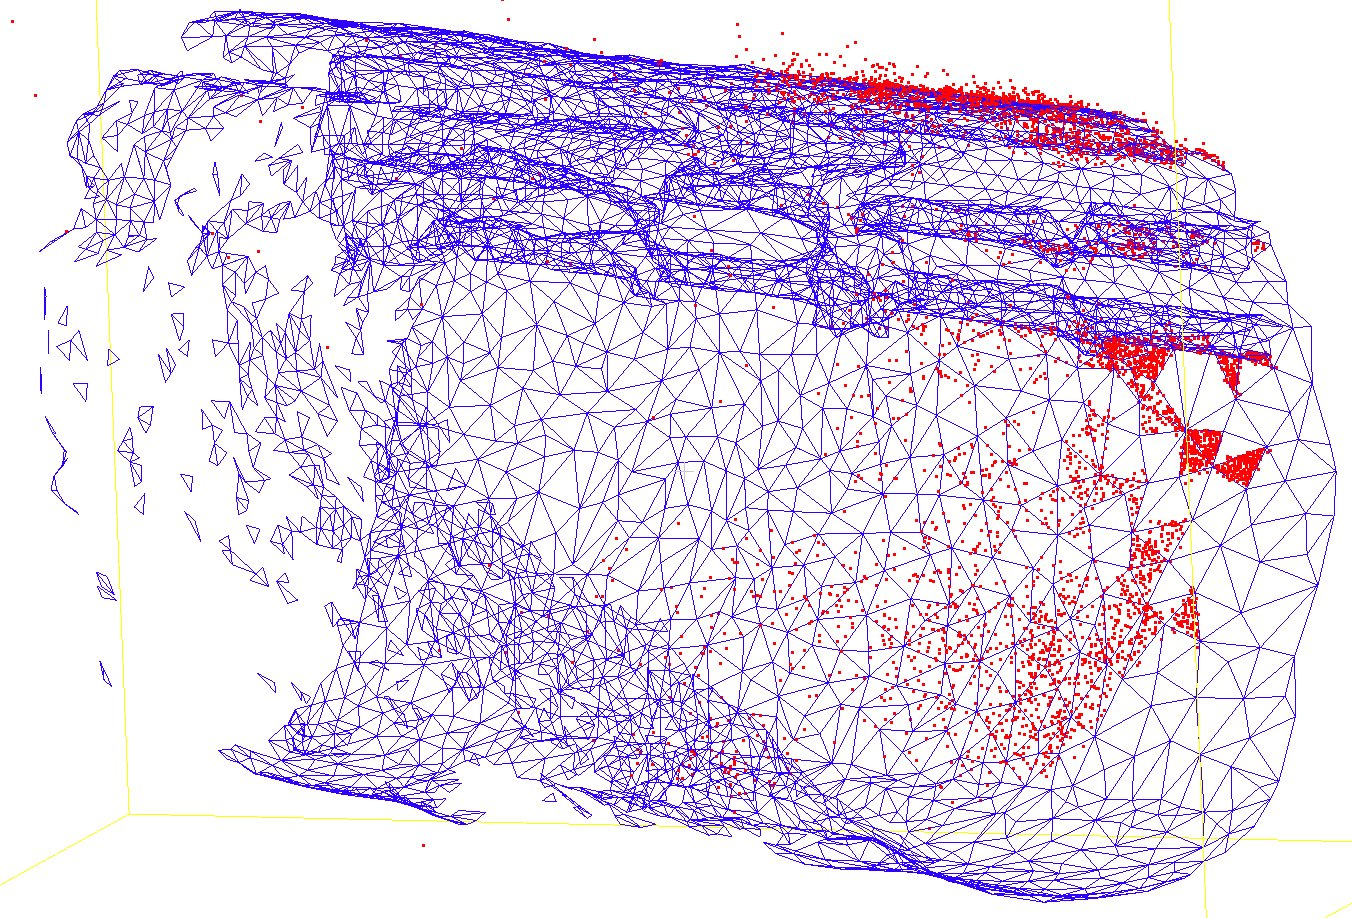
\includegraphics[width=15cm]{FIGS/MeshProjOnImg/TiePOnMesh.jpeg}
\caption{Draw tie point on mesh.}
\label{SurfCorr}
\end{figure}


%------------------------%
\subsection{MeshProjOnImg}
Tool use to back-project a mesh 3D on image 2D. Useful to specify which part of image is covered by the mesh.
Inputs:
\begin{itemize}
\item Pattern of image to examine.
\item Orientation of image
\item Mesh file.

\item zoomF : Zoom factor. Use to reduce image resolution to display. With image too big, display will cause program error. Default is 0.2, that's mean image is reduced to 1/5 of its size original.
\item click : Draw each triangle on mesh on image by mouse click. Each click will draw 1 triangle of mesh.
\end{itemize}
\textit{Attention:} Command will display all image of pattern at the same time, then reproject mesh on first image. You must click on first image to continue reproject mesh on second image and so on. When execute, command will read mesh file in and ask user if they like to display all the element in mesh file on the terminal. With "n", we can skip this step.

\begin{verbatim}
********************************************************
*               Reproject mesh on specific 	       *
********************************************************
*****************************
*  Help for Elise Arg main  *
*****************************
Mandatory unnamed args : 
  * string :: {Pattern of images}
  * string :: {Input Initial Orientation}
  * string :: {path to mesh(.ply) file - created by Inital Ori}
Named args : 
  * [Name=zoomF] REAL :: {1 -> sz origin, 0.2 -> 1/5 size - default = 0.2}
  * [Name=click] bool :: {true => draw each triangle by each click - default = false}
\end{verbatim}
\textit{Example:}
\textbf{mm3d MeshProjOnImg BIN\_010-011[1-4].*.tif Ori-BasculeIGN-sec01-21/ meshSimpleCut.ply}

\begin{figure}[H]
\centering
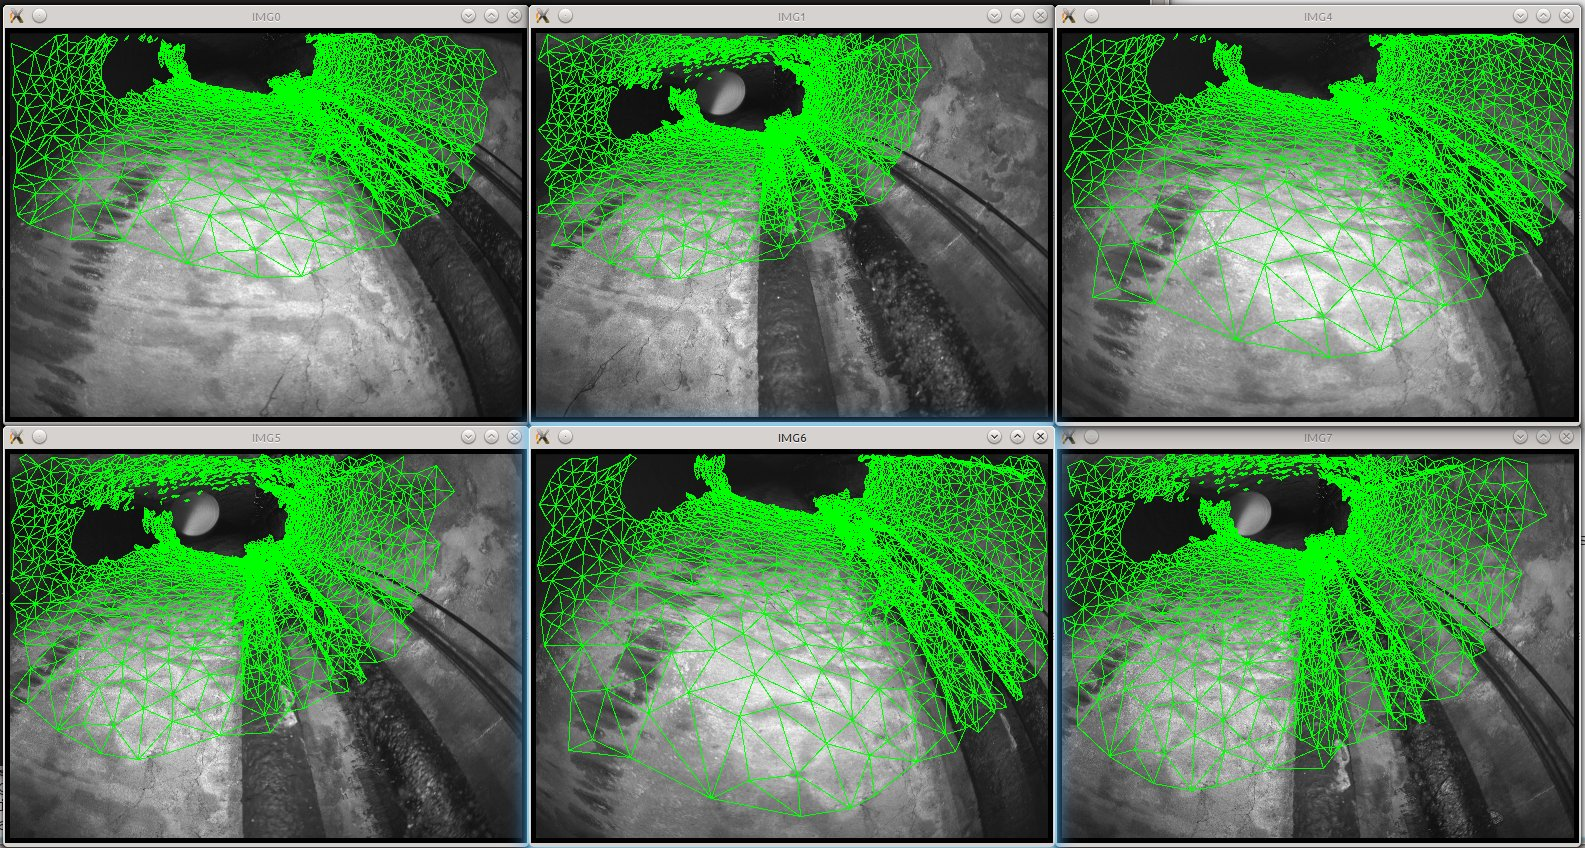
\includegraphics[width=15cm]{FIGS/MeshProjOnImg/meshOnImg.jpeg}
\caption{Result reproject mesh on image.}
\label{SurfCorr}
\end{figure}

%------------------------%
\subsection{InitOriLinear}

With {\tt InitOriLinear}, you can initialize your orientation in case of your acqusition is a serie of image with a displacement linear. Tool compute a vector of displacement from a set of reference image, then using it to estimate position of other image in serie.

By using this tool to initialize orientation before compute aero with Tapas, computation speed is improved.

Inputs:
\begin{itemize}
\item Folder contain orientation of reference images
\item Folder to output orientation file
\item Pattern of image need to initialize. If your system have many camera ona bar rigide, you can give pattern correspondant with each camera, seperate by ",".
\item Pattern of image use for reference. Idem if system have many camera. Order of camera must be the same.

\item PatTurn : Turn image when direction of acquisition changed.(new section) (image of 1st camera)
\item PatAngle : Turn angle correspondant with each turn image. Positive value for turn left, negative for turn right.
\item mulF : multiplication factor to adjustment position between each section (use to spread or shorten distance between section)
\item Axe : axe to turn around.
\end{itemize}

The output is orientation files initialized. Can be use as an initialized solution for {\tt Tapas} with option {\tt InOri}

\begin{verbatim}
mm3d InitOriLinear -help
************************
*  X : Initial         *
*  X : Orientation     *
*  X : & Position      *
*  X : For Acquisition *
*  X : Linear          *
************************
*****************************
*  Help for Elise Arg main  *
*****************************
Mandatory unnamed args : 
  * string :: {Ori folder of reference images}
  * string :: {Folder for output initialized orientation- default = Ori-InitOut}
  * string :: {Pattern of new images to orientate PatCam1, PatCam2,..}
  * string :: {Pattern of Reference Image = PatRef1, PatRef2,..}
Named args : 
  * [Name=PatTurn] vector<std::string> :: {Images when acquisition have turn [poseTurn1,poseTurn2...]}
  * [Name=PatAngle] vector<std::string> :: {Turn angle [angle1,angle2,...] - + => turn left, - => turn right}
  * [Name=mulF] vector<std::string> :: {Multiplication factor for adjustment each turn [mul1,mul2,...]}
  * [Name=Axe] string :: {Which axe to calcul rotation about - default = z}
  * [Name=WithIdent] bool :: {Initialize with orientation identique (default = false)}
  * [Name=Plan] bool :: {Force using vector [0,0,1] to initialize (garantie all poses will be in a same plan) - (default = false)}
\end{verbatim}

\underline{\textit{\textbf{Example:}}}

An acqutision with 3 section continue. Each section is seperate by a turn. Section 1, then turn left 90° to section 2, then turn left 45° to section 3 (Fig 7.7). Acqusition is done by a system 2 camera on a bar rigide.
Name image is contain an indicator of camera:
\begin{verbatim}
For camera 1: BIN_.*_image_023_.*.tif
For camera 2: BIN_.*_image_024_.*.tif
\end{verbatim}
Two turns in acqusition: 
\begin{verbatim}
Turn 1 : 90° left at image BIN_010-0120_14576019095_image_023_001_01316.thm.tif
Turn 2 : 45° left at image BIN_021-0150_14576061046_image_023_003_02935.thm.tif
\end{verbatim}

\underline{\textit{\textbf{Step 1:}}} orientate some images as a reference. Select image from 2 camera, in same shot to compute relative position between cameras and vector of displacement.
\begin{verbatim}
mm3d Tapas FishEyeBasic "BIN_010-011[1-2].*.tif" Out=reference
\end{verbatim}
We have an aero of reference image as show on Fig7.8.

\underline{\textit{\textbf{Step 2:}}} Initialize another image. We have 2 serie correspondant with 2 camera, and we have 2 turn. By using command {\tt InitOriLinear}:
\begin{verbatim}
mm3d InitOriLinear Ori-reference Ori-InitOut \
    "BIN_0.*-(011[4-9]|01[2-6]).*_023.*.tif,BIN_0.*-(011[4-9]|01[2-6]).*_024.*.tif" \
    "BIN_010-011[1-3].*_023.*.tif,BIN_010-011[1-3].*_024.*.tif" \
    PatTurn=[BIN_021-0128_14576060714_image_023_003_02913.thm.tif, \
             BIN_021-0148_14576061016_image_023_003_02933.thm.tif] \
    PatAngle=[90,45] mulF=[1,1] Axe=z
\end{verbatim}

In the command, we use orientation reference in Ori-reference, we have 2 pattern correspondant with 2 camera, first is 023 and seconde is 024. Acquisition turned at pose "BIN\_021-0128\_14576060714\_image\_023\_003\_02913.thm.tif" and "BIN\_021-0148\_14576061016\_image\_023\_003\_02933.thm.tif" with angle correspondant is 90° and 45°. Attention: number of image in each serie must be the same, and image to indicate a turn must be image of the first camera.
Result is shown on Fig7.8 and Fig7.9

\begin{figure}[H]
\centering
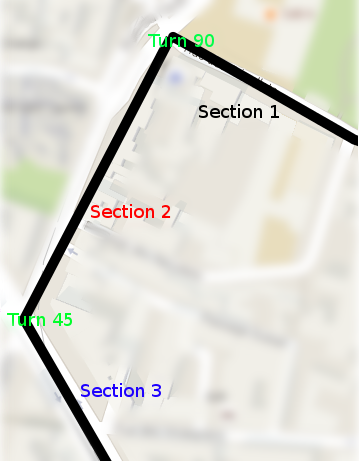
\includegraphics[width=4cm]{FIGS/InitOriLinear/planpartir_quartier.png}
\caption{Plan of acquisition linear with 2 turn, 3 section}
\label{SurfCorr}
\end{figure}
\begin{figure}[H]
\centering
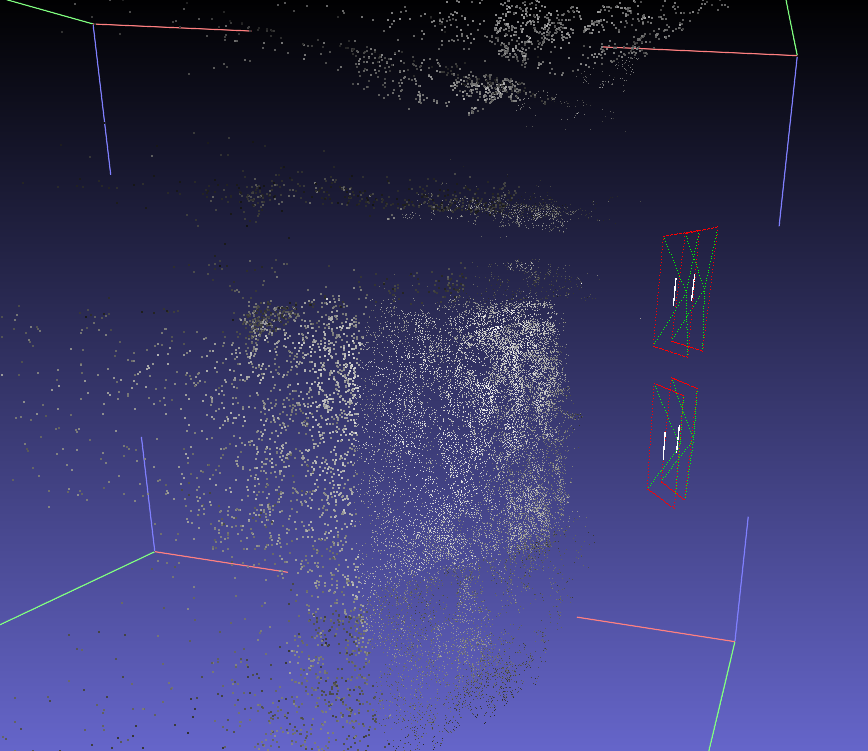
\includegraphics[width=10cm]{FIGS/InitOriLinear/InitPose01.png}
\caption{Calcul aero of reference image. System with 2 camera}
\label{SurfCorr}
\end{figure}
\begin{figure}[H]
\centering
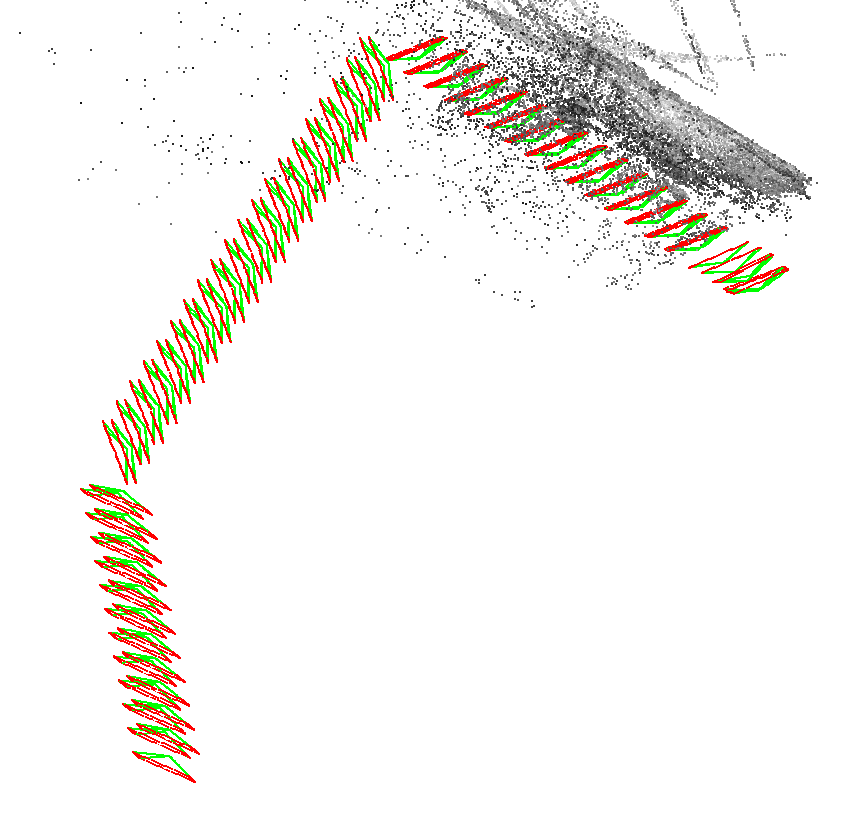
\includegraphics[width=10cm]{FIGS/InitOriLinear/InitAllImg2Turn00.png}
\caption{Result initialize oritentation of linear acquisition}
\label{SurfCorr}
\end{figure}
\begin{figure}[H]
\centering
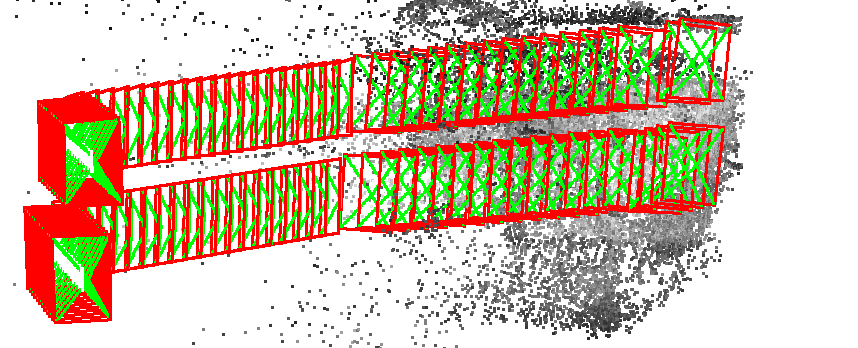
\includegraphics[width=10cm]{FIGS/InitOriLinear/InitAllImg2Turn01.png}
\caption{System with 2 camera}
\label{SurfCorr}
\end{figure}

%--------------------%
\subsection{ReprojImg}

With {\tt ReprojImg}, you can project an image into the orientation of an other.

Inputs:
\begin{itemize}
\item Two images (reference and projected image)
\item Ori of the two images
\item DEM of reference image
\end{itemize}

The output is the image reprojected into reference orientation.

\begin{verbatim}
mm3d ReprojImg -help
*****************************
*  Help for Elise Arg main  *
*****************************
Mandatory unnamed args : 
  * string :: {Orientation of reference image (xml)}
  * string :: {Reference DEM filename (xml)}
  * string :: {Reference image name}
  * string :: {Orientation of image to reproject (xml)}
  * string :: {Name of image to reproject}
Named args : 
  * [Name=AutoMask] string :: {AutoMask filename}
  * [Name=DepthRepImage] string :: {Image to reproject DEM file (xml), def=not used}
  * [Name=KeepLum] bool :: {Keep original picture luminosity (only for colorization), def=false}
\end{verbatim}

The {\tt KeepLum} argument is used to coloize reference picture, assuming that is green channel only.

As an example, when we have many pictures of first epoch (epoque1.*), we create a DEM,
then we can compute the orientation of an image of an other epoch (epoque2\_a.JPG) in the same reference,
and finally we reproject it in the (epoque1\_f.JPG) geometry :
\begin{verbatim}
mm3d Tapioca All "epoque1_..JPG" -1
mm3d Tapas RadialBasic "epoque1_..JPG"
mm3d Malt GeomImage "epoque1_..JPG" RadialBasic Master="epoque1_f.JPG"

mm3d Tapioca All "epoque._..JPG" -1
mm3d Tapas RadialBasic "epoque._..JPG" InOri=RadialBasic  Out=Tout

mm3d ReprojImg Ori-Tout/Orientation-epoque1_f.JPG.xml MM-Malt-Img-epoque1_f/Z_Num8_DeZoom1_STD-MALT.tif \
               epoque1_f.JPG Ori-Tout/Orientation-epoque2_a.JPG.xml epoque2_a.JPG
\end{verbatim}

%--------------------------%
\subsection{ExtractMesure2D}
The {\tt ExtractMesure2D} command extracts only a selection of targets in a 2D measures file. Its main purpose is to split images measures into used and check targets.

\begin{verbatim}
mm3d ExtractMesure2D -help
*****************************
*  Help for Elise Arg main  *
*****************************
Mandatory unnamed args : 
  * string :: {Input mes2D file}
  * string :: {Output mes2D file}
  * vector<std::string> :: {List of selected targets. Ex: [target1,target2])}
Named args : 
\end{verbatim}

Example:
\begin{verbatim}
mm3d ExtractMesure2D 21pts_Mesure-S2D.xml out.xml [3,203]
\end{verbatim}
Will save in out.xml only the 2D measures for targets 3 and 203.

%------------------------------%
\subsection{BasculeCamsInRepCam}
The {\tt BasculeCamsInRepCam} command express all images external parameters whith respect to the camera frame of one chosen image.

\begin{verbatim}
mm3d TestLib BasculeCamsInRepCam -help
*****************************
*  Help for Elise Arg main  *
*****************************
Mandatory unnamed args : 
  * string :: {Full Name (Dir+Pattern)}
  * string :: {Orientation}
  * string :: {Central camera}
  * string :: {Output}
\end{verbatim}

Example :
\begin{verbatim}
mm3d TestLib BasculeCamsInRepCam ".*JPG" Ori-AutoCal/ IMG00004.JPG Img04
\end{verbatim}

In {\tt Ori-Img04/} one can check that external parametrs of image {\tt IMG00004.JPG} are by definition equal to identity matrix.

%-----------------------------%
\subsection{BasculePtsInRepCam}
The {\tt BasculePtsInRepCam} command express coordinates of input points with respect to the camera frame of one chosen image.

\begin{verbatim}
mm3d TestLib BasculePtsInRepCam -help
*****************************
*  Help for Elise Arg main  *
*****************************
Mandatory unnamed args : 
  * string :: {Name Camera}
  * string :: {Name GGP In}
Named args : 
  * [Name=Out] string
\end{verbatim}

Example :
\begin{verbatim}
mm3d TestLib BasculePtsInRepCam Ori-AutoCal/Orientation-IMG00004.JPG.xml App.xml
\end{verbatim}

Output file {\tt Basc-Orientation-IMG00004.JPG-App.xml} contains points coordinates expressed in the camera frame of {\tt IMG00004.JPG}.

%-----------------%
\subsection{CorrLA}
The {\tt CorrLA} command computes corrected images positions with respect to a given value of lever-arm offset.

\begin{verbatim}
mm3d TestLib CorrLA -help
*****************************
*  Help for Elise Arg main  *
*****************************
Mandatory unnamed args : 
  * string :: {Full Name (Dir+Pattern)}
  * string :: {Directory orientation}
  * Pt3dr :: {Lever-Arm value}
Named args : 
  * [Name=OriOut] string :: {Output Ori Name of corrected mandatory Ori ; Def=OriName-CorrLA}
  * [Name=Ori2] string :: {Ori2 directory to apply LA correction to centers}
  * [Name=Ori2Out] string :: {Output Ori Name of corrected Ori2 ; Def=Ori2Name-CorrLA}
\end{verbatim}

Example:
\begin{verbatim}
mm3d TestLib CorrLA ".*JPG" Ori-Basc/ [0.289,-0.043,-0.183] Ori2=Ori-Nav-GPS/
\end{verbatim}

Sometimes, it is more accurate to compute the lever-arm correction and to apply it to a second set of images positions.
Using the optional argument {\tt Name=Ori2} one can apply corrections calculated with the orientations from the mandatory {\tt Ori-Basc/} and generate {\tt Ori-Nav-GPS-CorrLA/} with
lever-arm corrected positions. 

%---------------------------%
\subsection{ExportXmlGcp2Txt}
The {\tt ExportXmlGcp2Txt} command simply convert a GCP .xml file format into a column format text file.

\begin{verbatim}
mm3d TestLib ExportXmlGcp2Txt -help
*****************************
*  Help for Elise Arg main  *
*****************************
Mandatory unnamed args : 
  * string :: {Directory}
  * string :: {xml Gcps file}
Named args : 
  * [Name=Out] string :: {output txt file name : def=Output.txt}
  * [Name=addInc] bool :: {export also uncertainty values : def=flase}
\end{verbatim}

Example :
\begin{verbatim}
mm3d TestLib ExportXmlGcp2Txt './' AppAll.xml Out=AppAll-Txt.txt
\end{verbatim}

This command can be useful for example when a GCP file is converted to .xml format using {\tt mm3d GCPConvert} with a change of system and the user wants to recover transformed coordinates in a simple format.


%------------------------%
\subsection{SimplePredict}
The {\tt SimplePredict} command projects ground points on oriented images.

\begin{verbatim}
mm3d SimplePredict -help
*****************************
*  Help for Elise Arg main  *
*****************************
Mandatory unnamed args : 
  * string :: {Pattern of images}
  * string :: {Directory orientation}
  * string :: {Ground points file}
Named args : 
  * [Name=ExportPolyIGN] bool :: {Export PointeInitIm files for IGN Polygon calibration method (Def=false)}
  * [Name=PrefixeNomImageSize] INT :: {Size of PrefixeNomImage in param.txt}
\end{verbatim}

Example :
\begin{verbatim}
mm3d SimplePredict ".*JPG" Ori-Basc/ AppAll.xml
\end{verbatim}

The output {\tt SimplePredict.xml} file contains (i,j) coordinates of all {\tt AppAll.xml} points in all possible images.

%---------------------%
\subsection{Export2Ply}
The {\tt Export2Ply} command generates a .ply file containing spheres to represent points.

\begin{verbatim}
mm3d TestLib Export2Ply -help
*****************************
*  Help for Elise Arg main  *
*****************************
Mandatory unnamed args : 
  * string :: {Format specification}
  * string :: {Name File of Points Coordinates}
Named args : 
  * [Name=Ray] REAL :: {Plot a sphere per point}
  * [Name=NbPts] INT :: {Number of Pts / direc (Def=5, give 1000 points) only with Ray > 0}
  * [Name=Scale] INT :: {Scaling factor}
  * [Name=FixColor] Pt3di :: {Fix the color of points}
  * [Name=LastPtColor] Pt3di :: {Change color only for last point}
  * [Name=ChangeColor] INT :: {Change the color each number of points : not with FixColor}
  * [Name=Out] string :: {Default value is NameFile.ply}
  * [Name=Bin] INT :: {Generate Binary or Ascii (Def=1, Binary)}
\end{verbatim}

Example :
\begin{verbatim}
mm3d TestLib Export2Ply "#F=N_X_Y_Z" AppAll-Txt.txt Ray=0.5 FixColor=[0,0,255]
\end{verbatim}

This is sometimes useful for example when one wants to represent GCPs into a point cloud to clearly visualize its distribution.

%--------------------------%
\subsection{PseudoIntersect}
The {\tt PseudoIntersect} command estimates the 3D position coordinates of 2D measured points in oriented images.

\begin{verbatim}
mm3d TestLib PseudoIntersect -help
*****************************
*  Help for Elise Arg main  *
*****************************
Mandatory unnamed args : 
  * string :: {Full Name (Dir+Pat)}
  * string :: {Directory of input orientation}
  * string :: {.xml file of 2d points}
Named args : 
  * [Name=Out] string :: {Name output file (def=3DCoords.txt)}
  * [Name=XmlOut] bool :: {Export in .xml format to use as GCP file (Def=true)}
  * [Name=Show] bool :: {Gives details on arguments (Def=true)}
\end{verbatim}

Example :
\begin{verbatim}
mm3d TestLib PseudoIntersect ".*JPG" Ori-All/ MesuresFinales-S2D.xml
\end{verbatim}

Each point needs to be measured at least in 2 images to compute an intersection.
The output .xml file can be directly used as a GCP file with {\tt GCPBascule} tool.

%--------------------------%
\subsection{MasqMaker}
The {\tt MasqMaker} command create masks for each picture to remove too dark or too light areas.

\begin{verbatim}
*****************************
*  Help for Elise Arg main  *
*****************************
Mandatory unnamed args : 
  * string :: {Pattern images}
  * INT :: {Minimum value}
  * INT :: {Maximum value}
Named args : 
  * [Name=MasqSup] string :: {Supplementary mask}
  * [Name=SzW] INT :: {SzW for masking (def=0)}
\end{verbatim}

It is useful to avoid correlation in burned areas.


%--------------------------%
\subsection{SkyMask}

The {\tt SkyMask} tool (in {\tt Testlib}) creates masks for each image to remove sky areas. It has two main purposes: \newline

\begin{itemize}
	\item remove sky tie points with \texttt{HomolFilterMasq}
	\item remove non-sky line of sights of GNSS observations with \texttt{ExcludeSats} \newline
\end{itemize}

\begin{verbatim}
*****************************
*  Help for Elise Arg main  *
*****************************
Mandatory unnamed args : 
* string :: {Image pattern}
* string :: {Output folder}
Named args : 
* [Name=Prob] string :: {Probabilistic prediction}
* [Name=Thresh] string :: {Decision threshold}
* [Name=Inv] string :: {Inverse prediction}
* [Name=Filter] string :: {Filtering (artifacts relative size)}
* [Name=Install] string :: {Install neural net program}
* [Name=Uninstall] string :: {Uninstall neural net program}
\end{verbatim}

\noindent \texttt{SkyMask} relies on Python neural network, so it must be installed before first usage. It is recommended to use a Python virtual environment (venv). Installation steps are described hereafter (assuming Python is already installed). \newline

\noindent In the working directory, create and activate a virtual environment with the following instructions: \newline

\begin{verbatim}
python -m venv .venv
source .venv/bin/activate 
\end{verbatim}

\noindent If the activation was successful, the prompt should start with \texttt{(.venv)} header. It is recommended to upgrade python package installer (pip) with the command: \newline

\begin{verbatim}
pip install --upgrade pip
\end{verbatim}

\noindent Installation of \texttt{SkyMask} neural network may be automatically carried out with the \texttt{Install} optional argument of \texttt{SkyMask} command set to \texttt{1}. During this step, all the mandatory arguments may be set to arbitrary values: \newline

\begin{verbatim}
mm3d TestLib SkyMask 1 1 Install=1
\end{verbatim}

\noindent This command line should process the following tasks (assuming internet network is available): \newline


\begin{itemize}
	\item download python neural network code (\texttt{predict.py})
	\item download neural network model parameters (\texttt{best\_model.h5})
	\item install python necessary packages:  \texttt{TensorFlow}, \texttt{Keras}, \texttt{albumentations} and \texttt{segmentation-models}. \newline
\end{itemize}

\noindent The tool \texttt{SkyMask} is then installed in \texttt{home/.local/share/mm3d/skymask} folder\footnote{Note that this folder is used as well to store temporary images, but it is cleaned at the end of process.}. It is possible to uninstall it with: \newline

\begin{verbatim}
mm3d TestLib SkyMask 1 1 Uninstall=1
\end{verbatim}

\noindent Once \texttt{SkyMask} is succesfully installed, and the virtual environment is activated, it is possible to detect sky in images (for example here with \textit{Vincennes castle} datset) with the base command: \newline

\begin{verbatim}
mm3d TestLib SkyMask "Calib-IMGP52.*.JPG" sky
\end{verbatim}

\noindent Images are first reduced (to the nominal size of $480\times360$ px), then sky area is detected with dense convolutional neural network and eventually some further post-processing steps (posterior probabilities equalization, automatic thresholding, connex refinement, etc) are performed before turning back the images to their original size. Note that all input images may have different number of pixels. \newline

\begin{figure}[!h]
	\begin{center}
		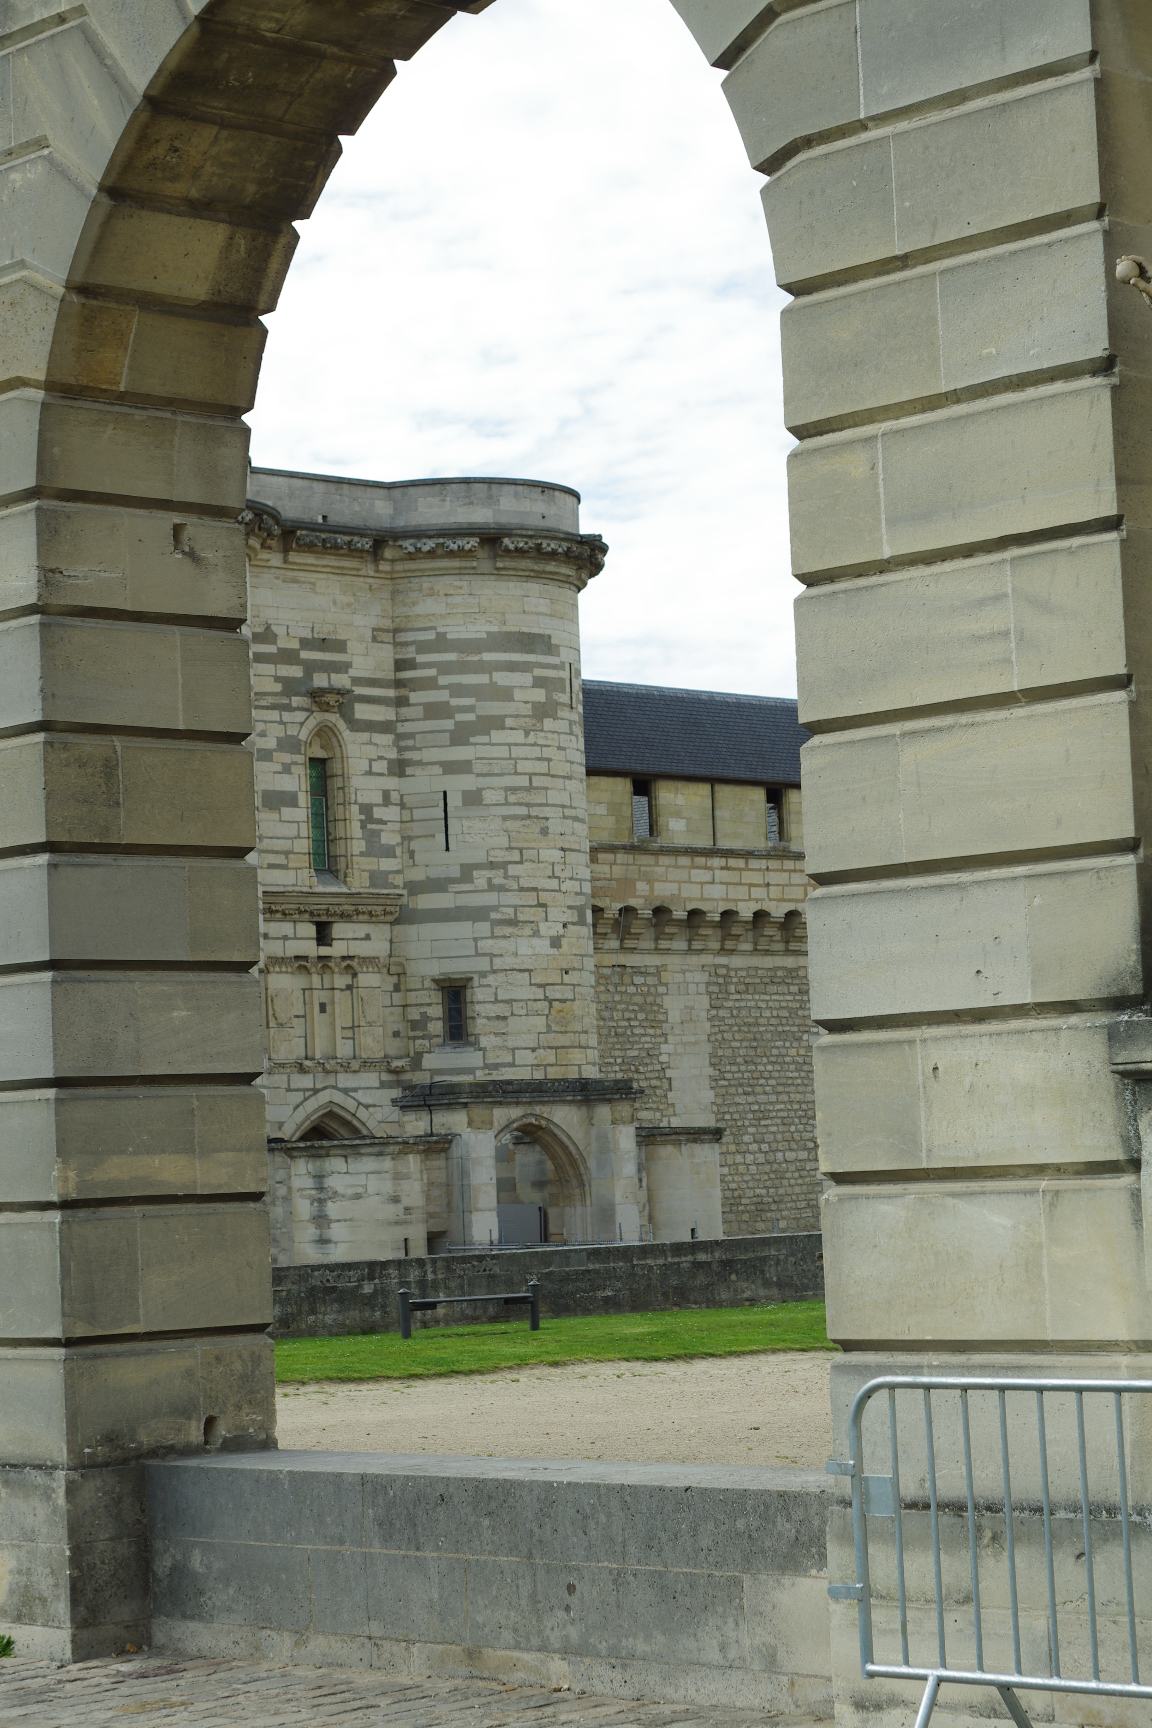
\includegraphics[width=40mm]{FIGS/SkyMask/im1.JPG}
		\hspace{0.2cm}
		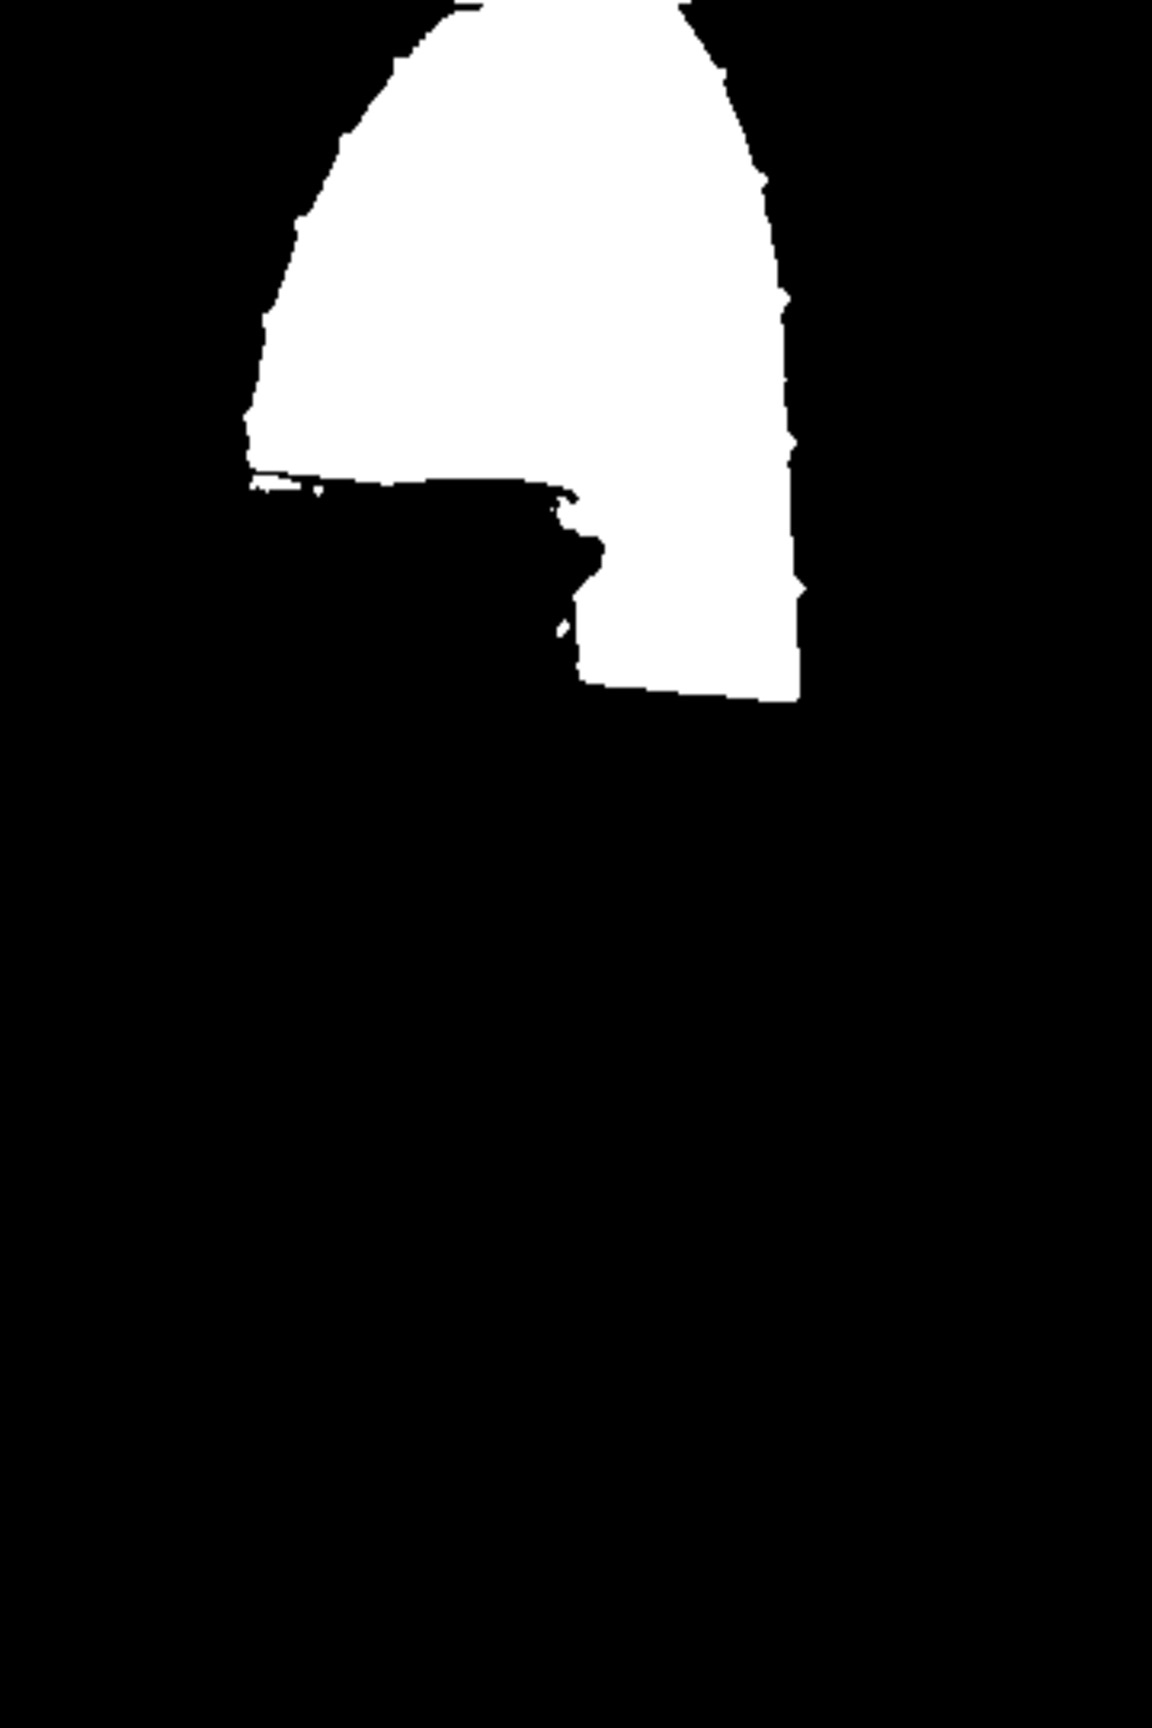
\includegraphics[width=40mm]{FIGS/SkyMask/mask1.JPG}
		\caption{Original image (left) and binary sky mask inference (right).}
	\end{center}	
\end{figure}


\noindent For typical image sizes ($1500 \times 1500$ px), processing speed is about 1000 images per hour (for an Intel Core(TM) i7-3770 CPU @ 3.40GHz). \newline

\noindent After using \texttt{SkyMask}, the virtual environment may be shut down with \texttt{deactivate} command. If necessary, it can be suppressed with \texttt{rm -r .venv}. \newline

\noindent \texttt{SkyMask} performs quite well, even on moderately challenging situations. On stereopolis dataset (urban cloudy scenes), pixewise accuracy has been estimated to be up to 99.5 \%. \newline

\begin{figure}[!h]
	\begin{center}
		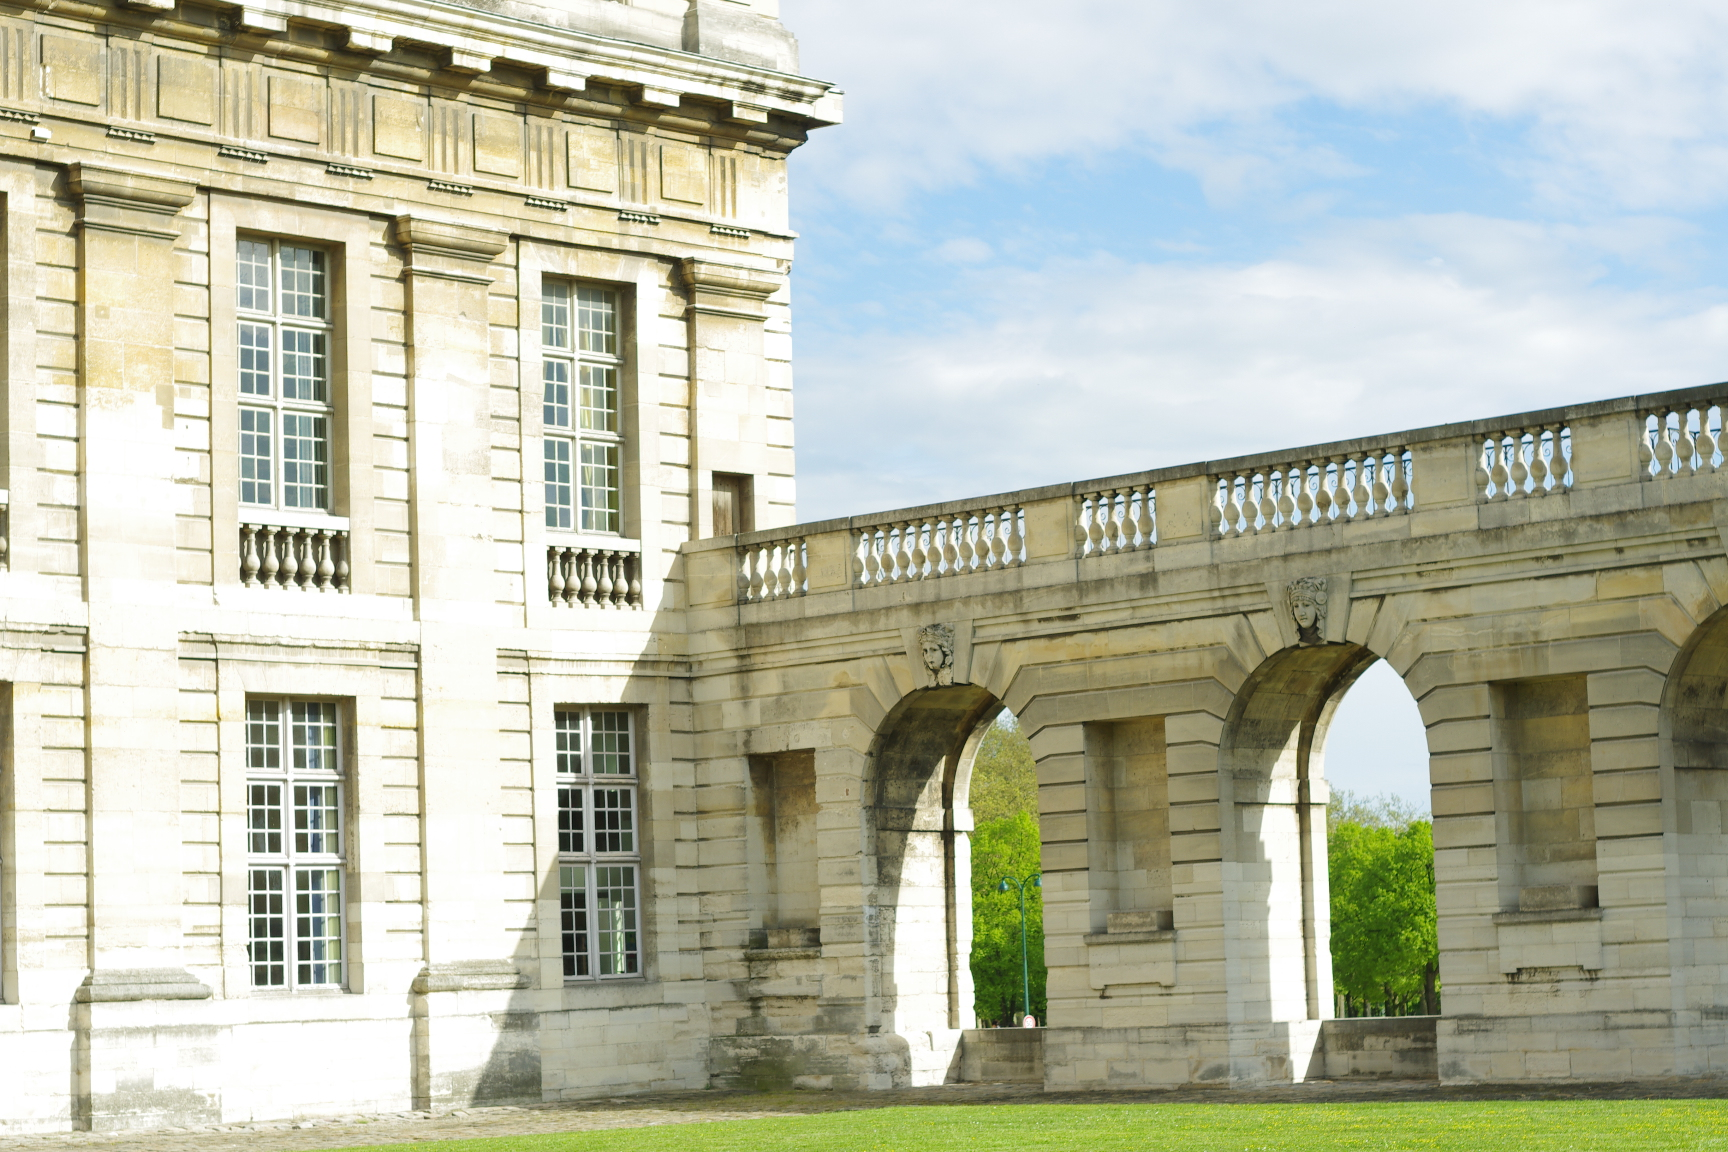
\includegraphics[width=70mm]{FIGS/SkyMask/im2.JPG}
		\hspace{0.2cm}
		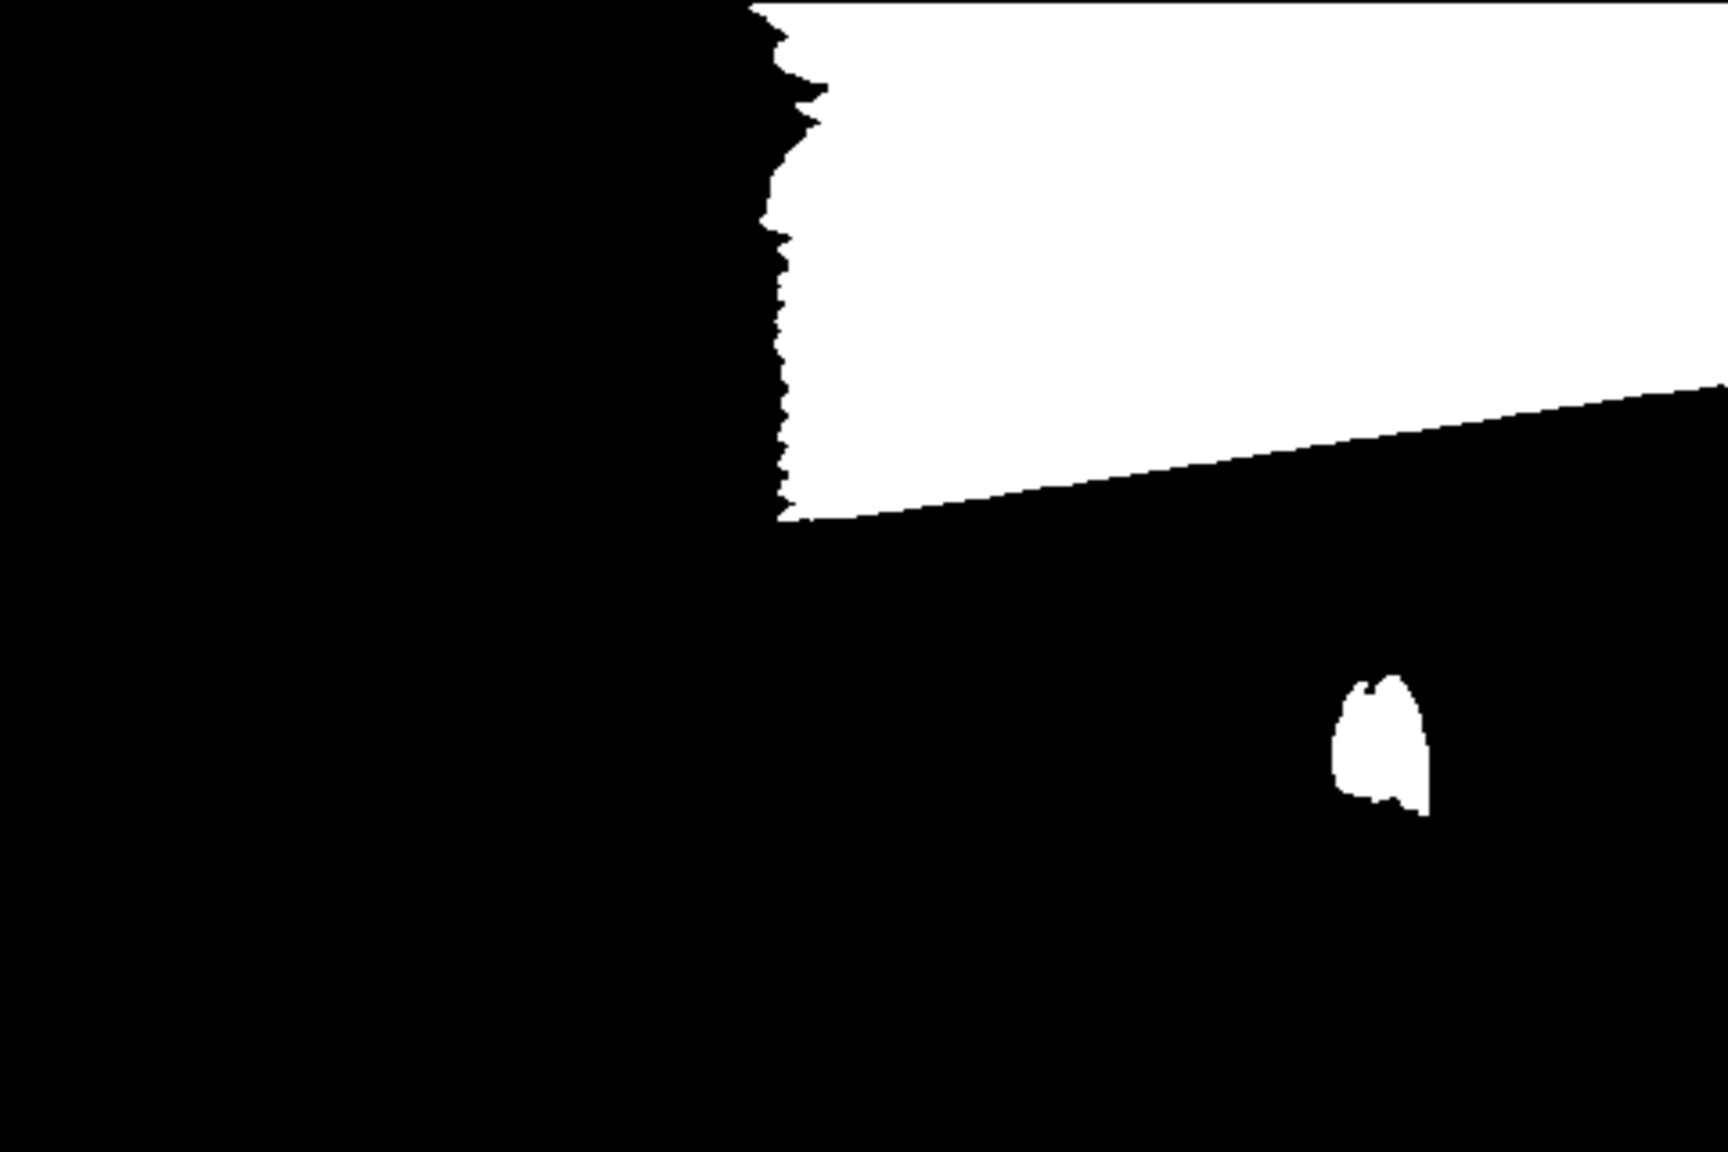
\includegraphics[width=70mm]{FIGS/SkyMask/mask2.JPG}
		\caption{Original image (left) and binary sky mask inference (right).}
	\end{center}	
\end{figure}

\noindent Regarding optional parameters of \texttt{SkyMask}: \newline

\begin{itemize}
	\item \texttt{Prob}: probabilistic prediction. Output is given in integer values between 0 and 255. When divided by 255, the value may be interpreted as the posterior probability for each pixel to be part of a sky area. \newline
	
	\begin{figure}[!h]
		\begin{center}
			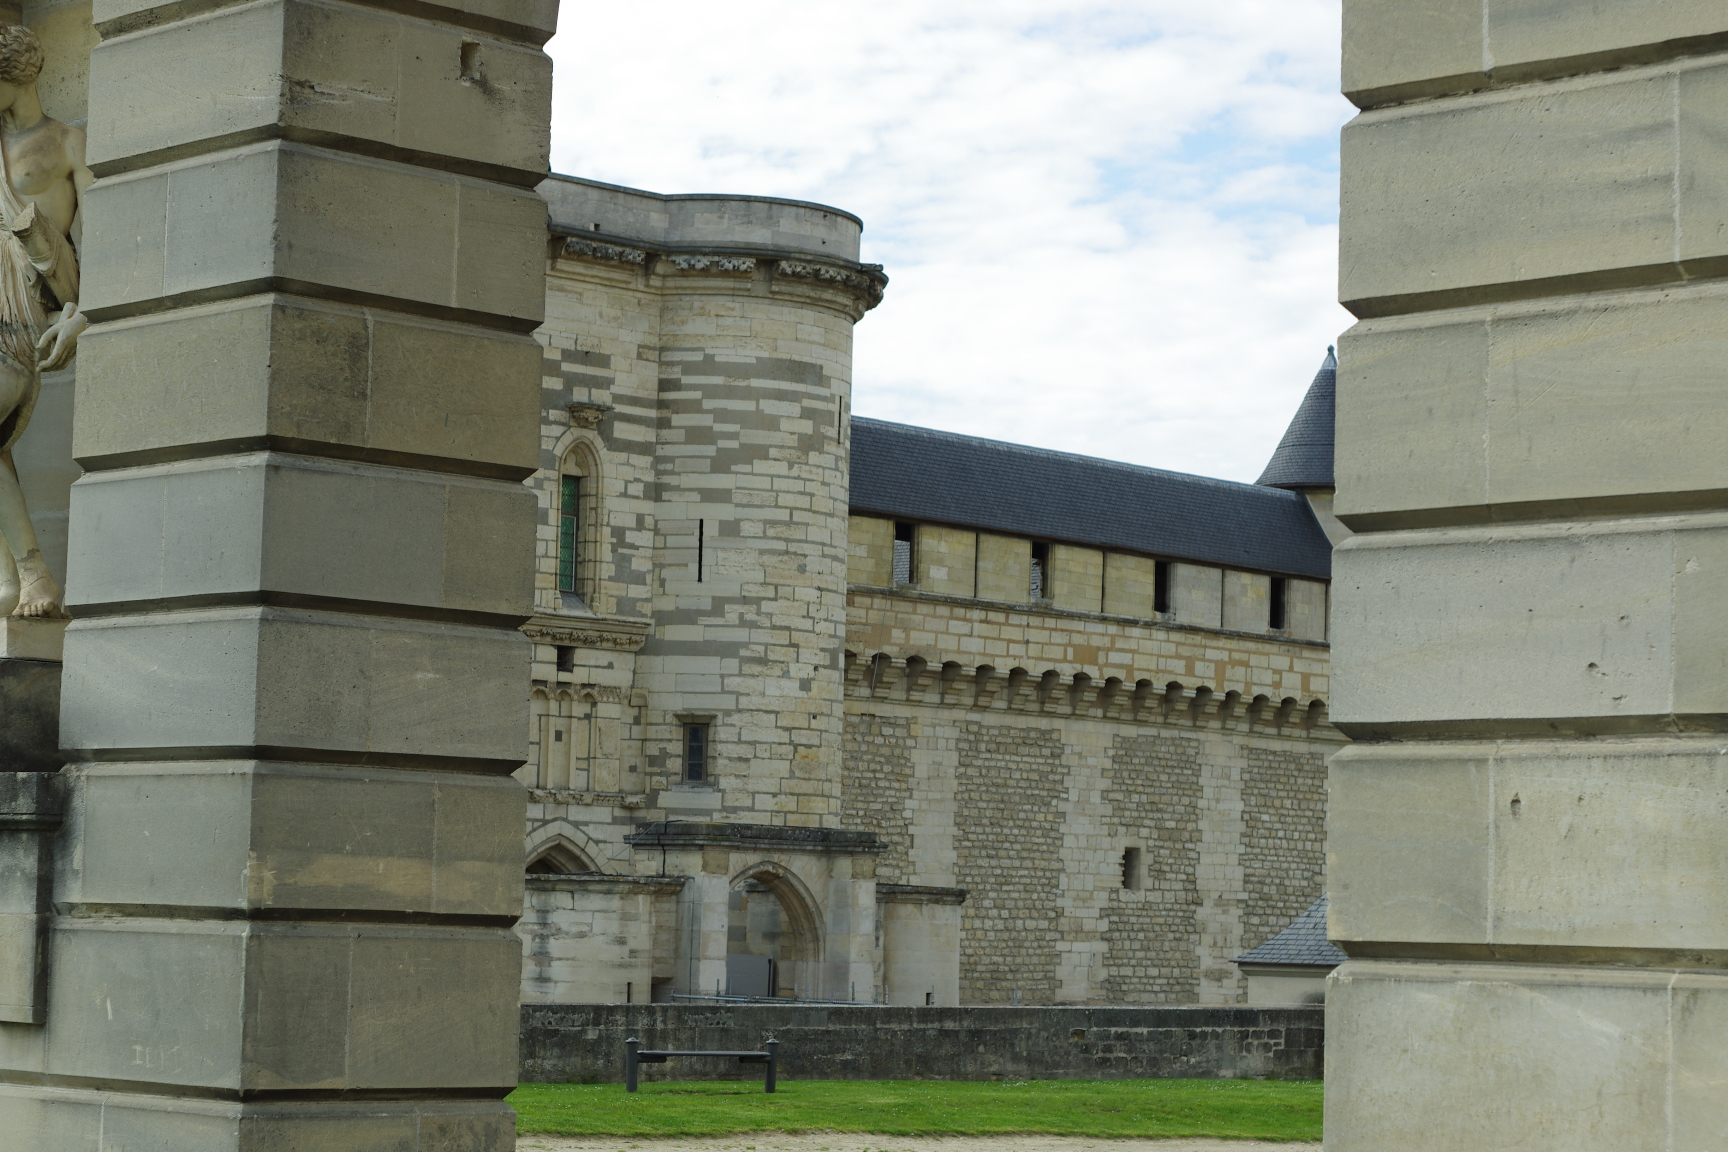
\includegraphics[width=70mm]{FIGS/SkyMask/im3.JPG}
			\hspace{0.2cm}
			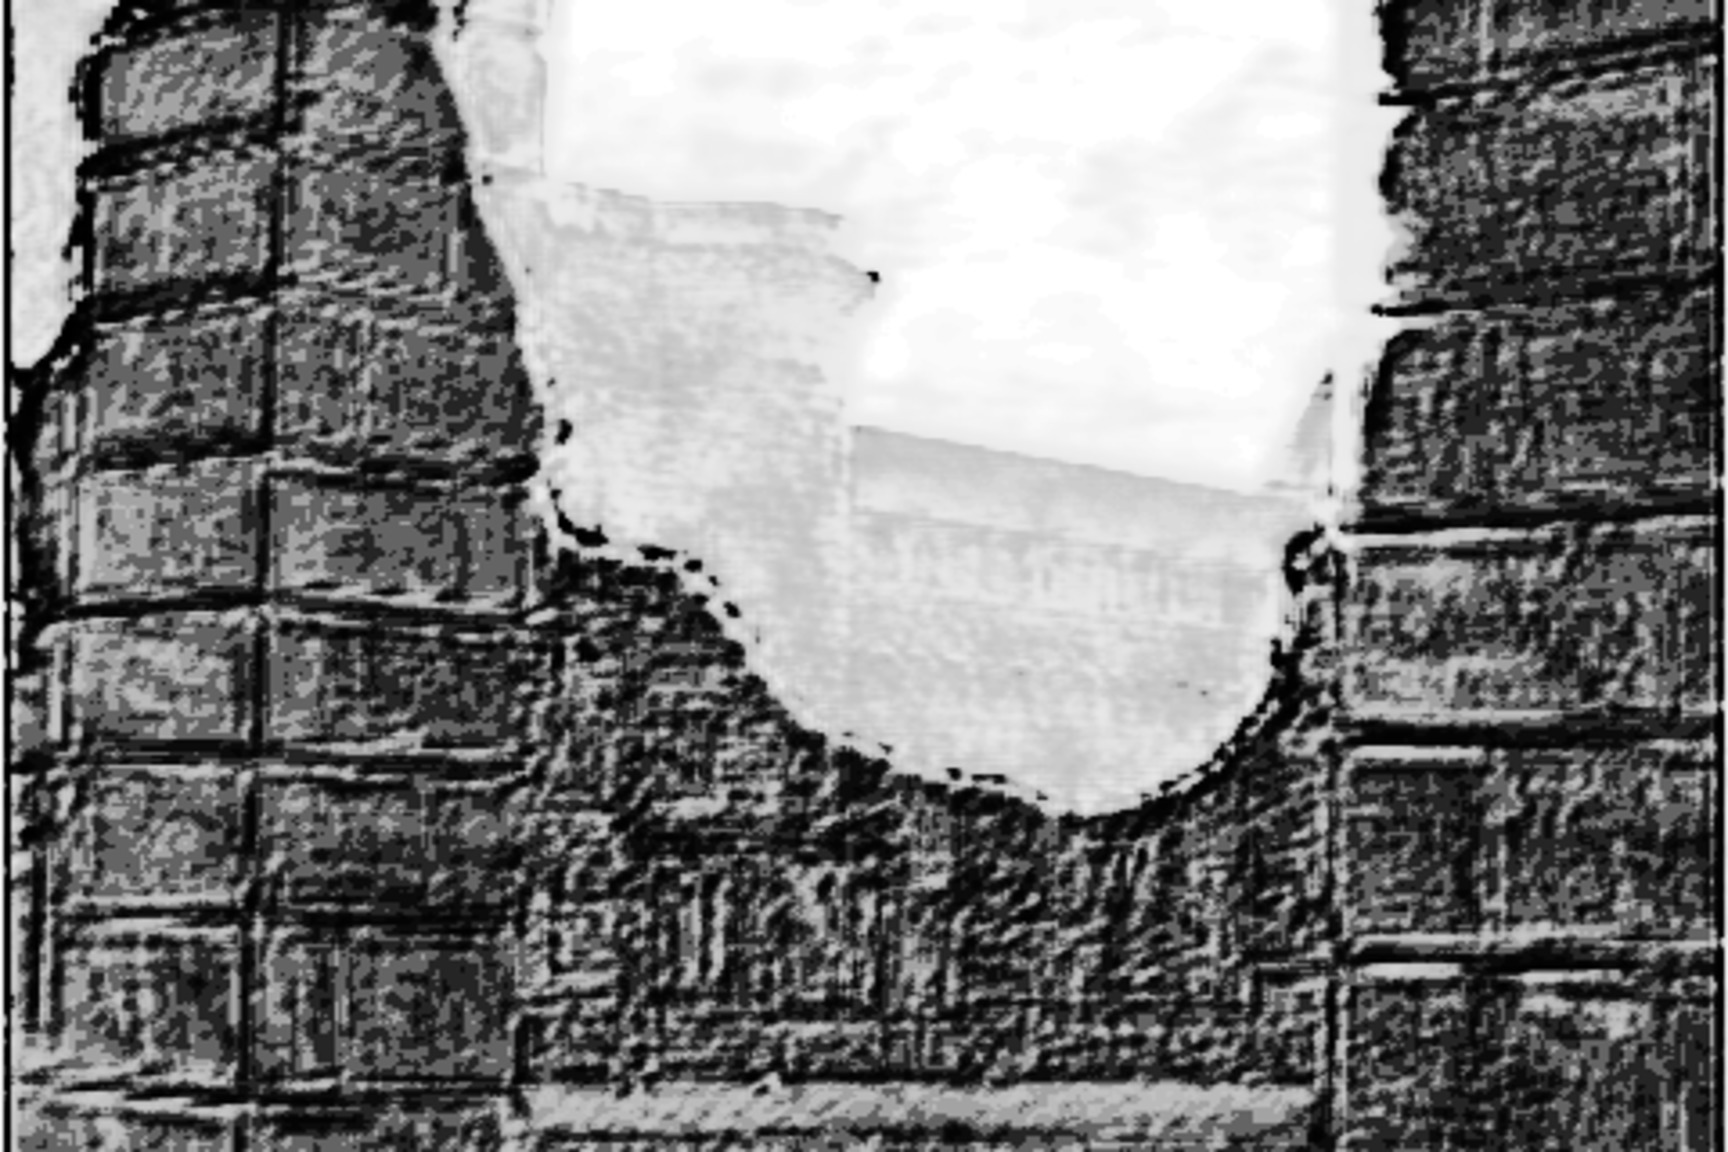
\includegraphics[width=70mm]{FIGS/SkyMask/mask3.JPG}
			\caption{Original image (left) and posterior probability sky mask inference (right).}
		\end{center}	
	\end{figure}
	
	\item \texttt{Thresh}: decision threshold is used to input a prior probability in the inference process. By default, threshold is set automatically to get exactly 50 \% of pixels (of the entire image dataset) in sky area. For example, a threshold value of 0.9 states that all pixels above $0.9 \times 255 \approx 230$ are classified as sky. Higher threshold values mean that ambiguous pixels tend to be more easily classified as non-sly areas. \newline
	
	\begin{figure}[!h]
		\begin{center}
			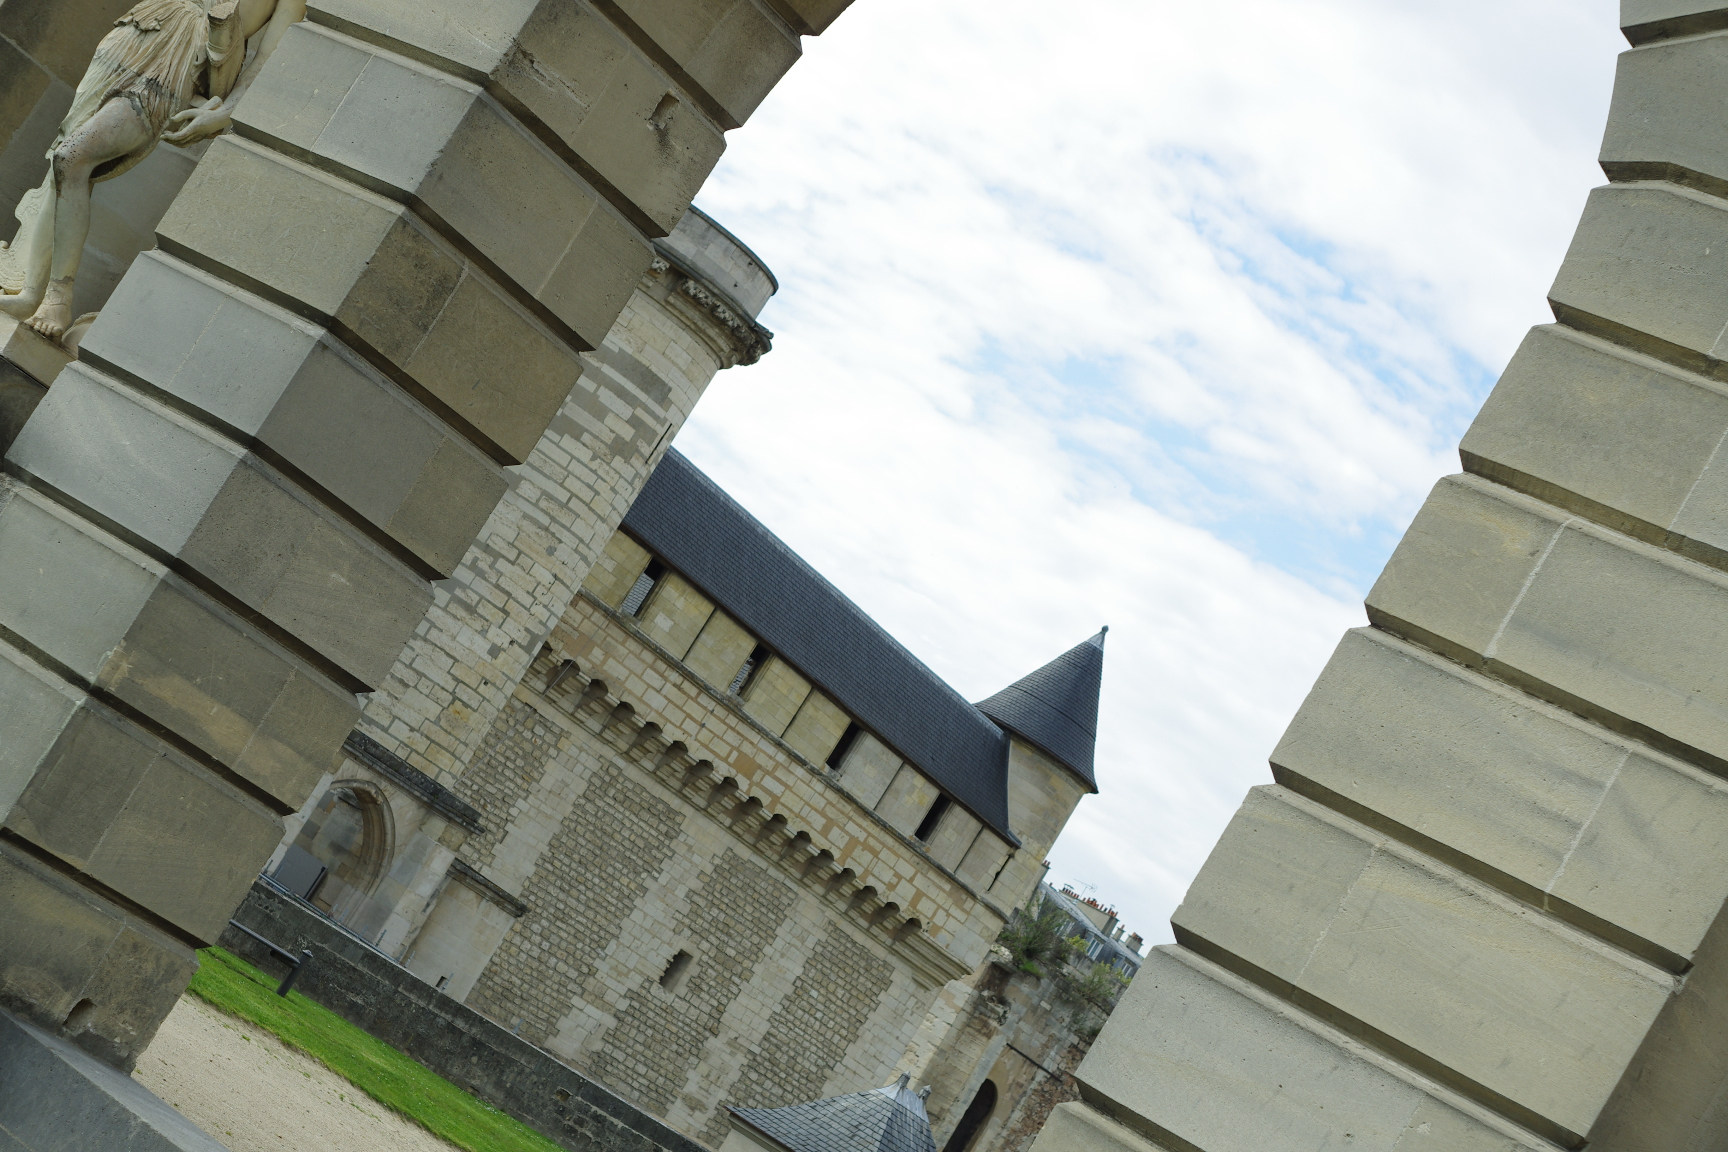
\includegraphics[width=40mm]{FIGS/SkyMask/im_thresh.JPG}
			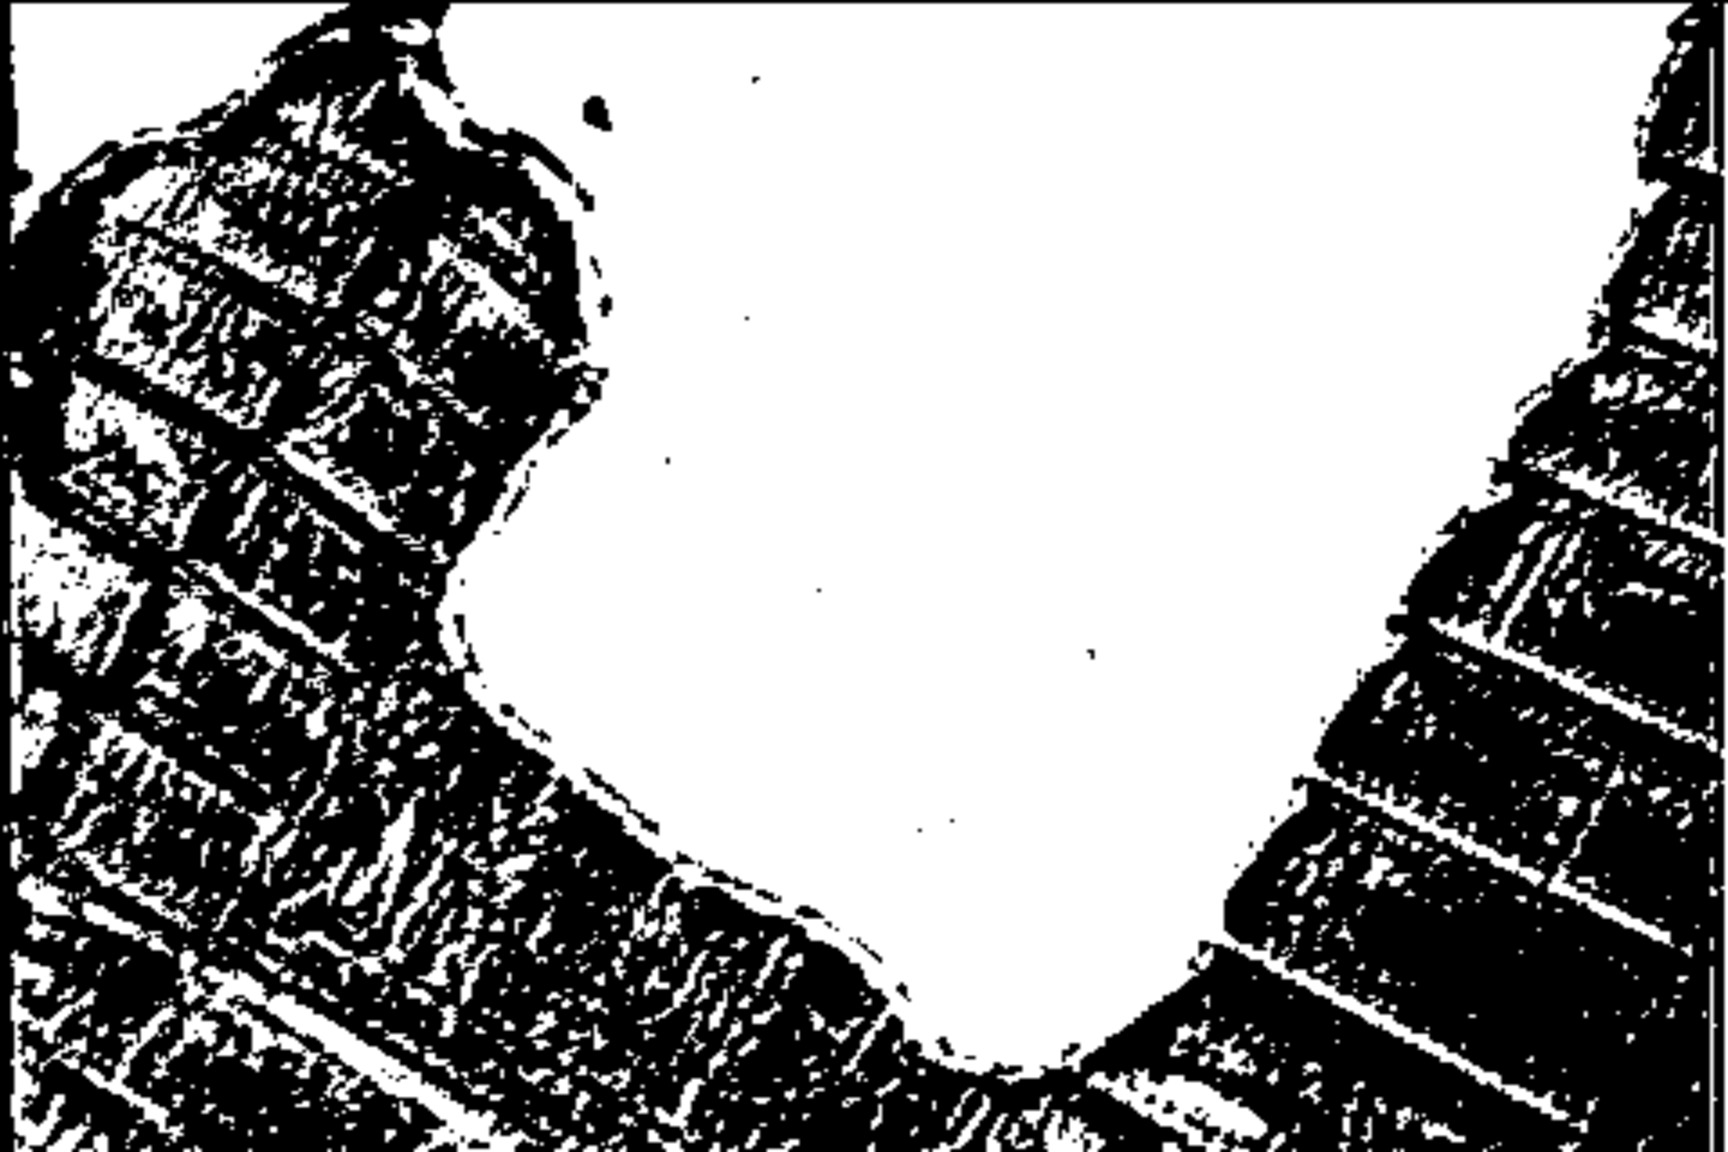
\includegraphics[width=40mm]{FIGS/SkyMask/im_thresh_40.JPG}
			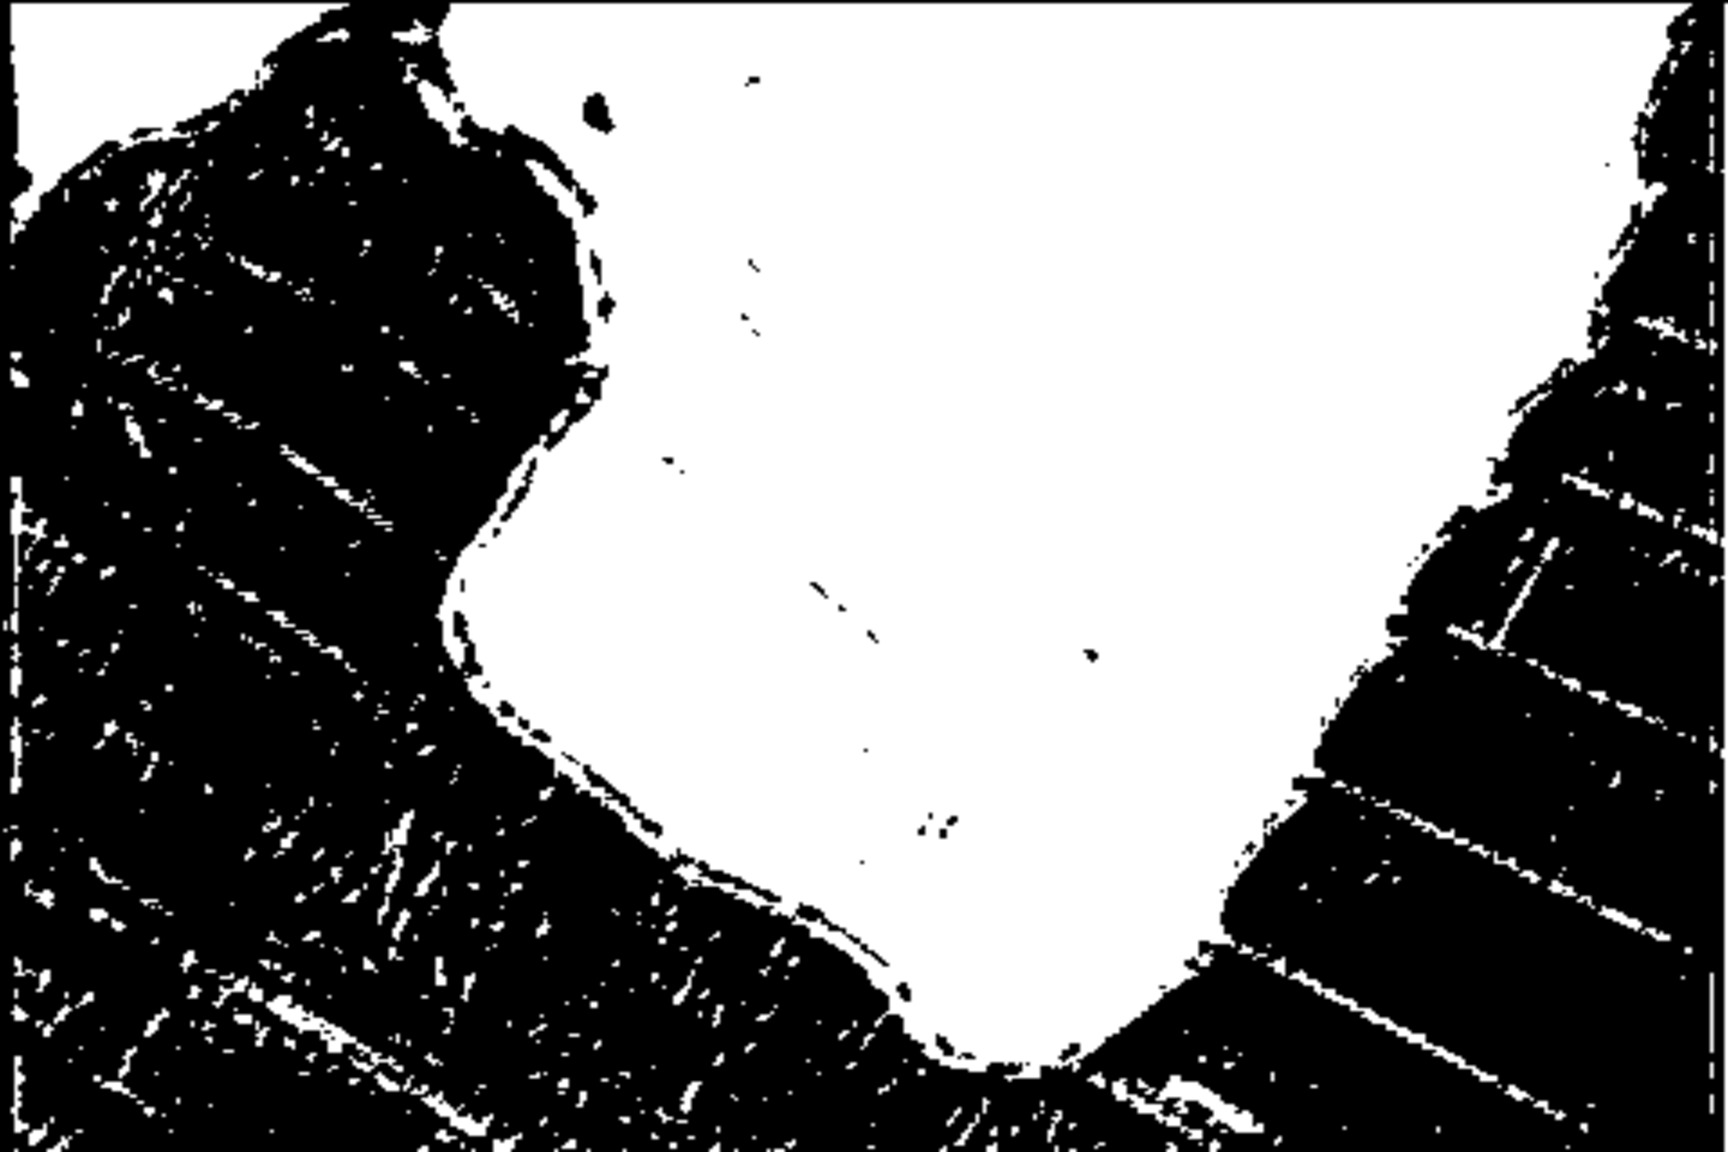
\includegraphics[width=40mm]{FIGS/SkyMask/im_thresh_50.JPG}
			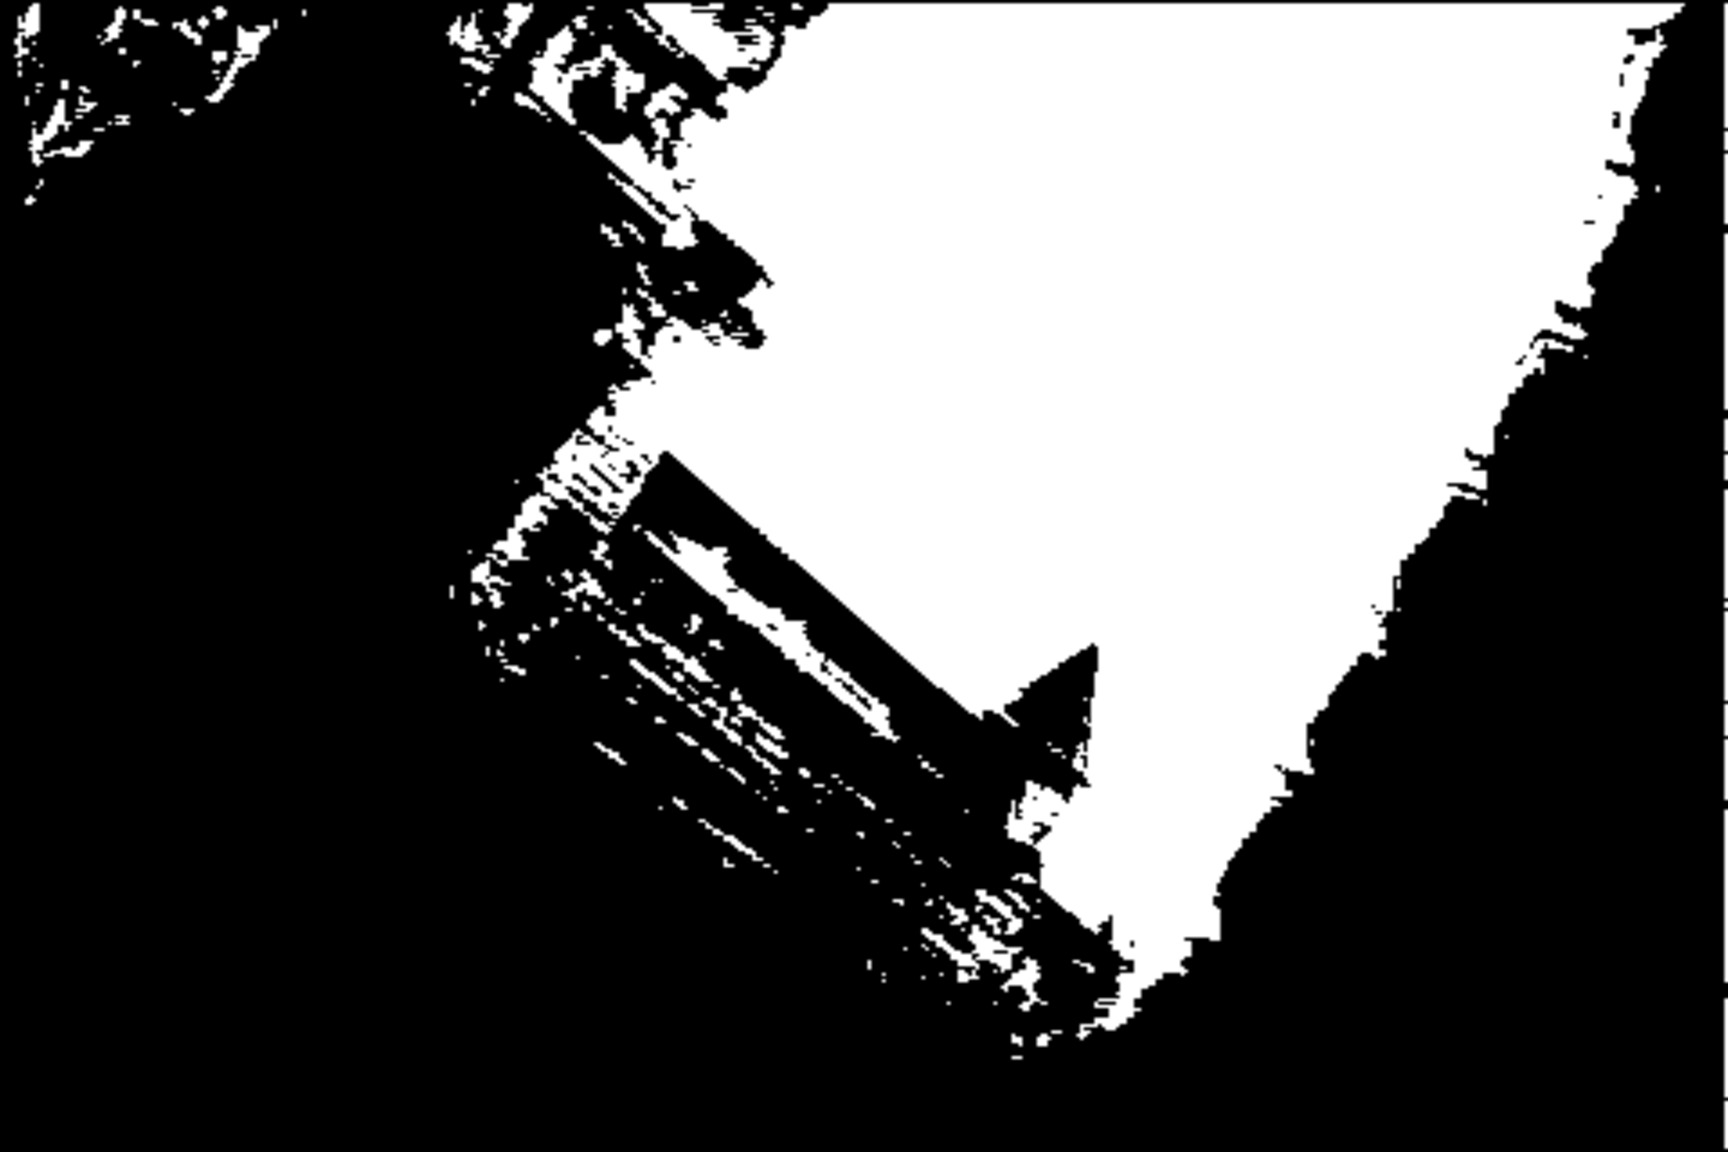
\includegraphics[width=40mm]{FIGS/SkyMask/im_thresh_70.JPG}
			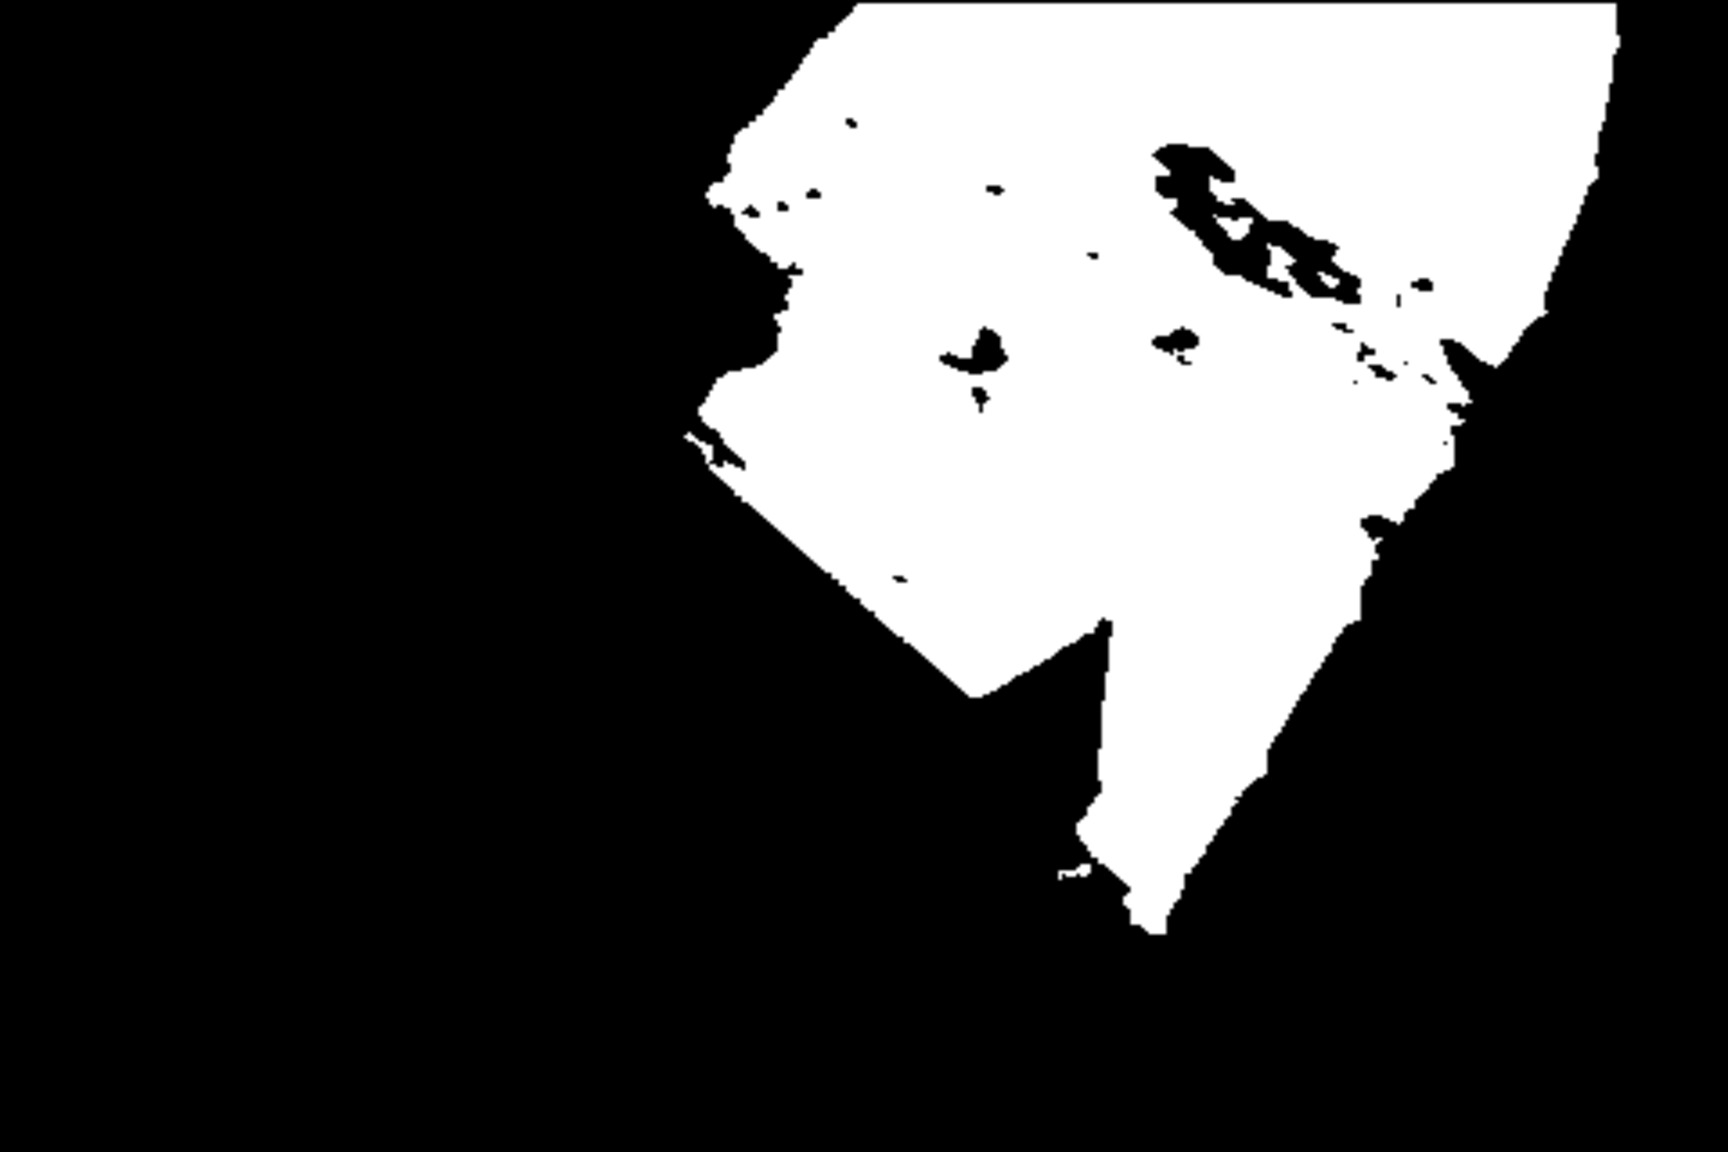
\includegraphics[width=40mm]{FIGS/SkyMask/im_thresh_80.JPG}
			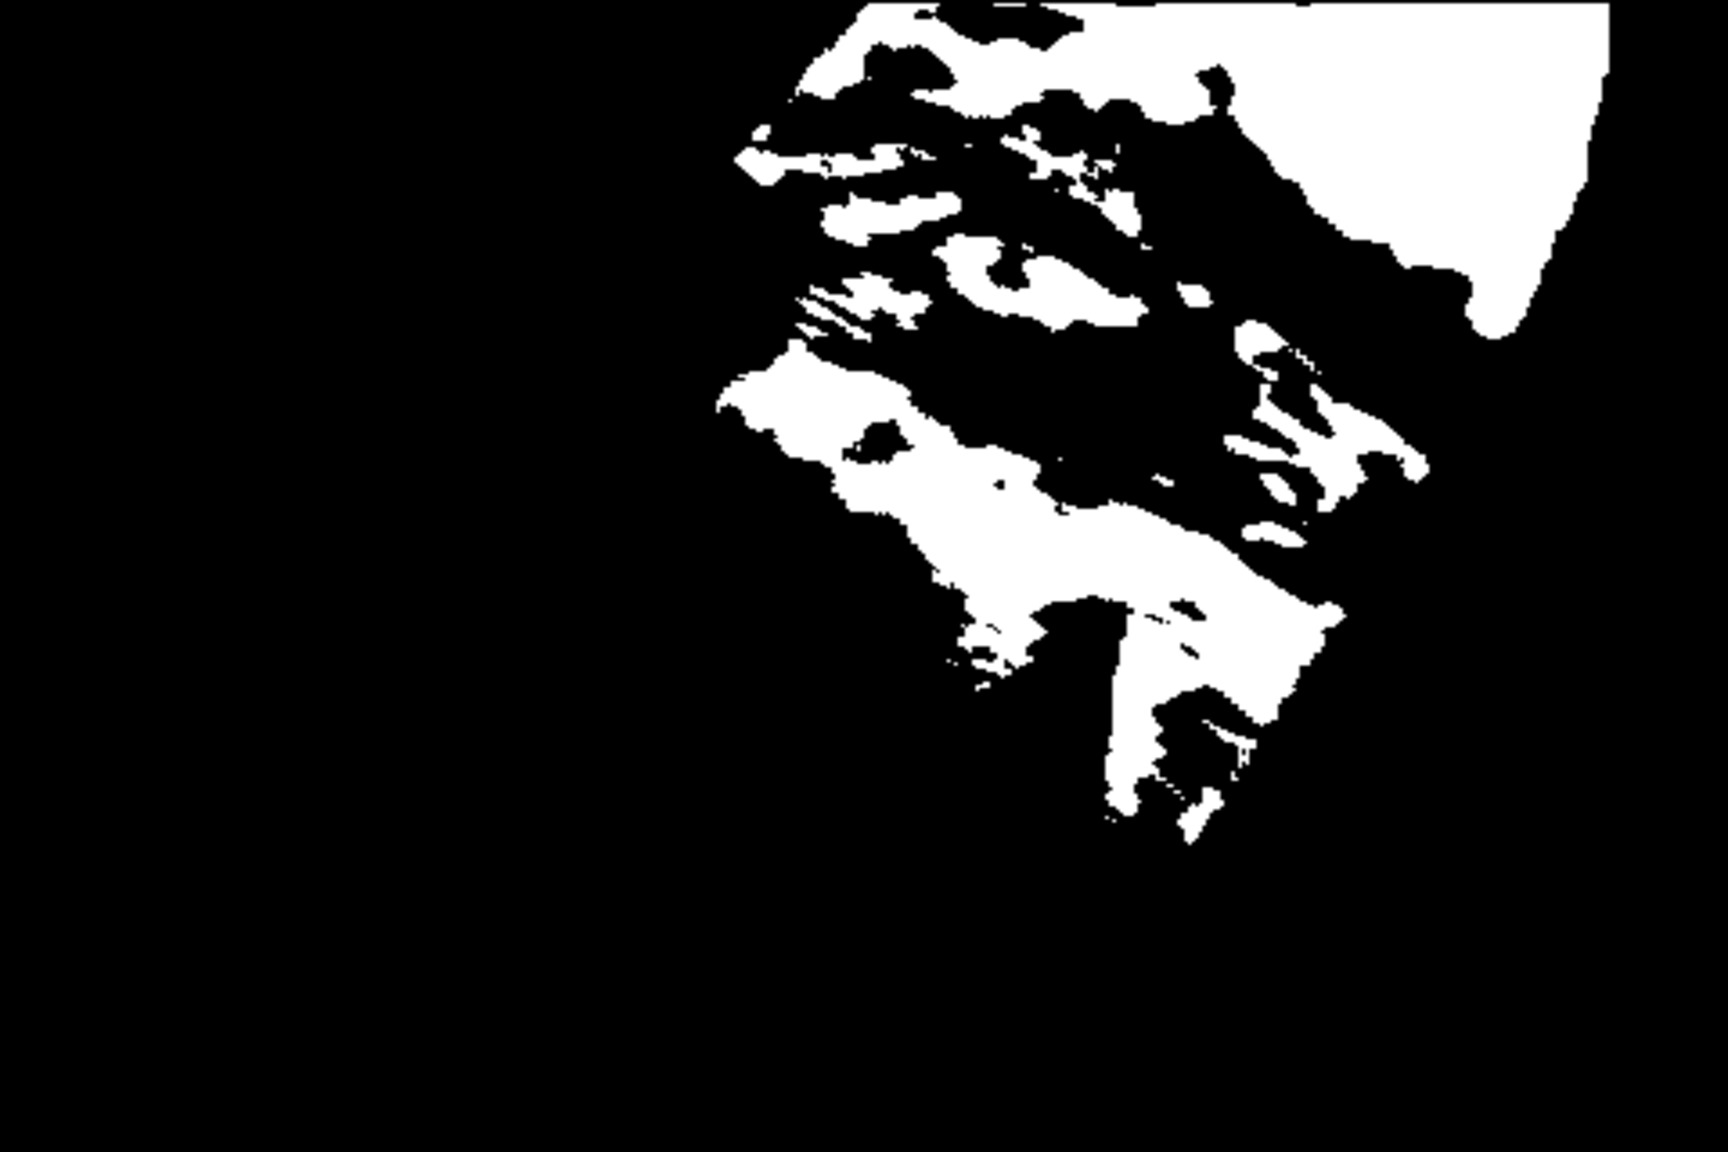
\includegraphics[width=40mm]{FIGS/SkyMask/im_thresh_90.JPG}
			\caption{From top to down, and left to right: original image and binary sky mask prediction for different thresholds (0.4, 0.5, 0.7, 0.8 and 0.9). The optimal threshold seems to be somewhere between 0.7 and 0.8.}
		\end{center}	
	\end{figure}
	
	\item  \texttt{Inv}: invert predicted values. Brighter values mean sky probability is lower. This option may be used with \texttt{HomolFilterMasq} to remove non-sky tie points, or in \texttt{ExcludeSats} to remove non-line of sight (NLOS) GNSS satellites from rinex observation file, for loosely-coupled GNSS-Images hybrid positioning solution. \newline
	
	\item \texttt{Filter}: removes small non-sky area connex components. The typical size (in image relative size) must be provided. For example, we can compare the results of the three following commands: \newline
	
	\begin{verbatim}
	mm3d TestLib SkyMask "Calib-IMGP5249.*.JPG" sky Thresh=0.8
	mm3d TestLib SkyMask "Calib-IMGP5249.*.JPG" sky Thresh=0.8 Filter=0.05
	mm3d TestLib SkyMask "Calib-IMGP5249.*.JPG" sky Thresh=0.8 Filter=0.10
	\end{verbatim}   
	
	\vspace{0.5cm}
	
	In the first case, no filtering is applied, then none of the artifacts in the center of the image are removed. In the second case, only non-sky connex components whose typical size is below 5\% of image dimensions. In this case, image size is $1728 \times 1152$, which means a typical size of $1500$. Therefore, only non-sky connex components of diameter up to $0.05 \times 1500 = 75$ px are filtered. We observe that one artifact is remaining after the process. In the third case, filtering is performed with parameter $0.1$, removing all artifacts. \newline
	
		\begin{figure}[!h]
		\begin{center}
			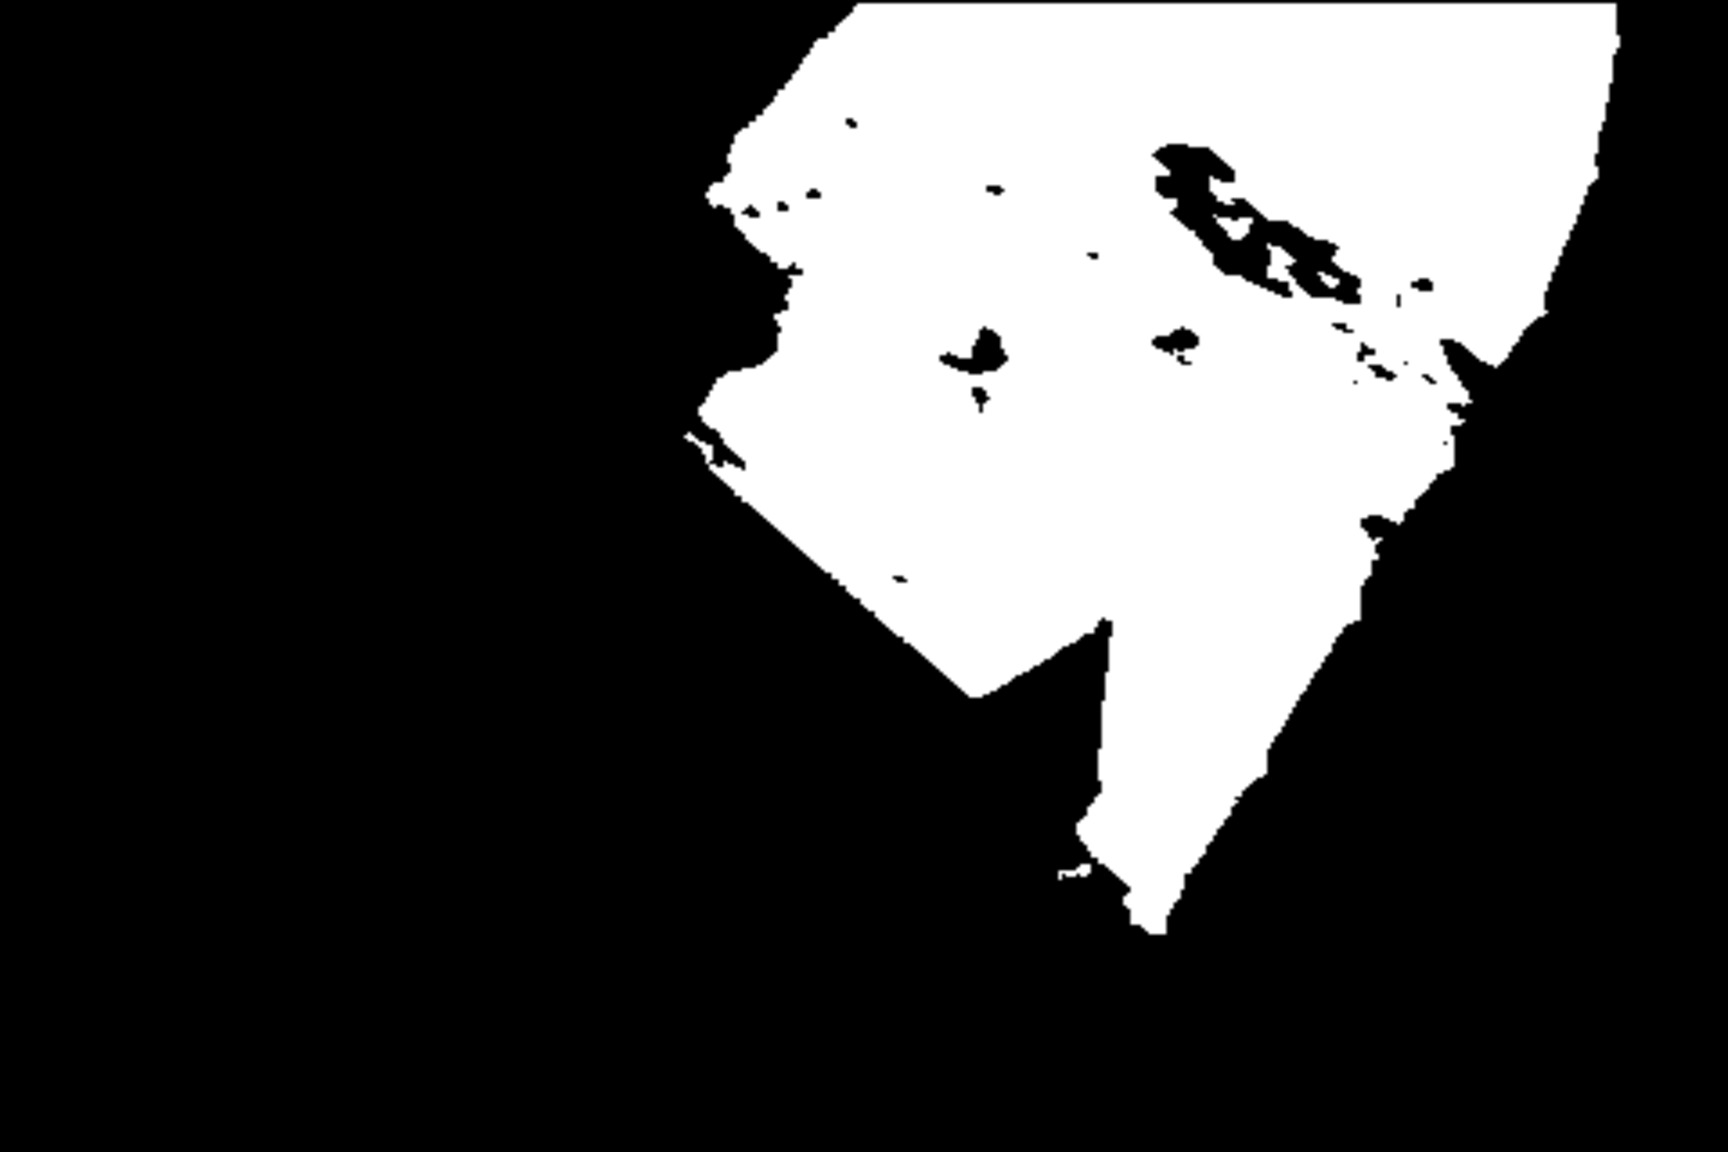
\includegraphics[width=40mm]{FIGS/SkyMask/im_px_0.JPG}
			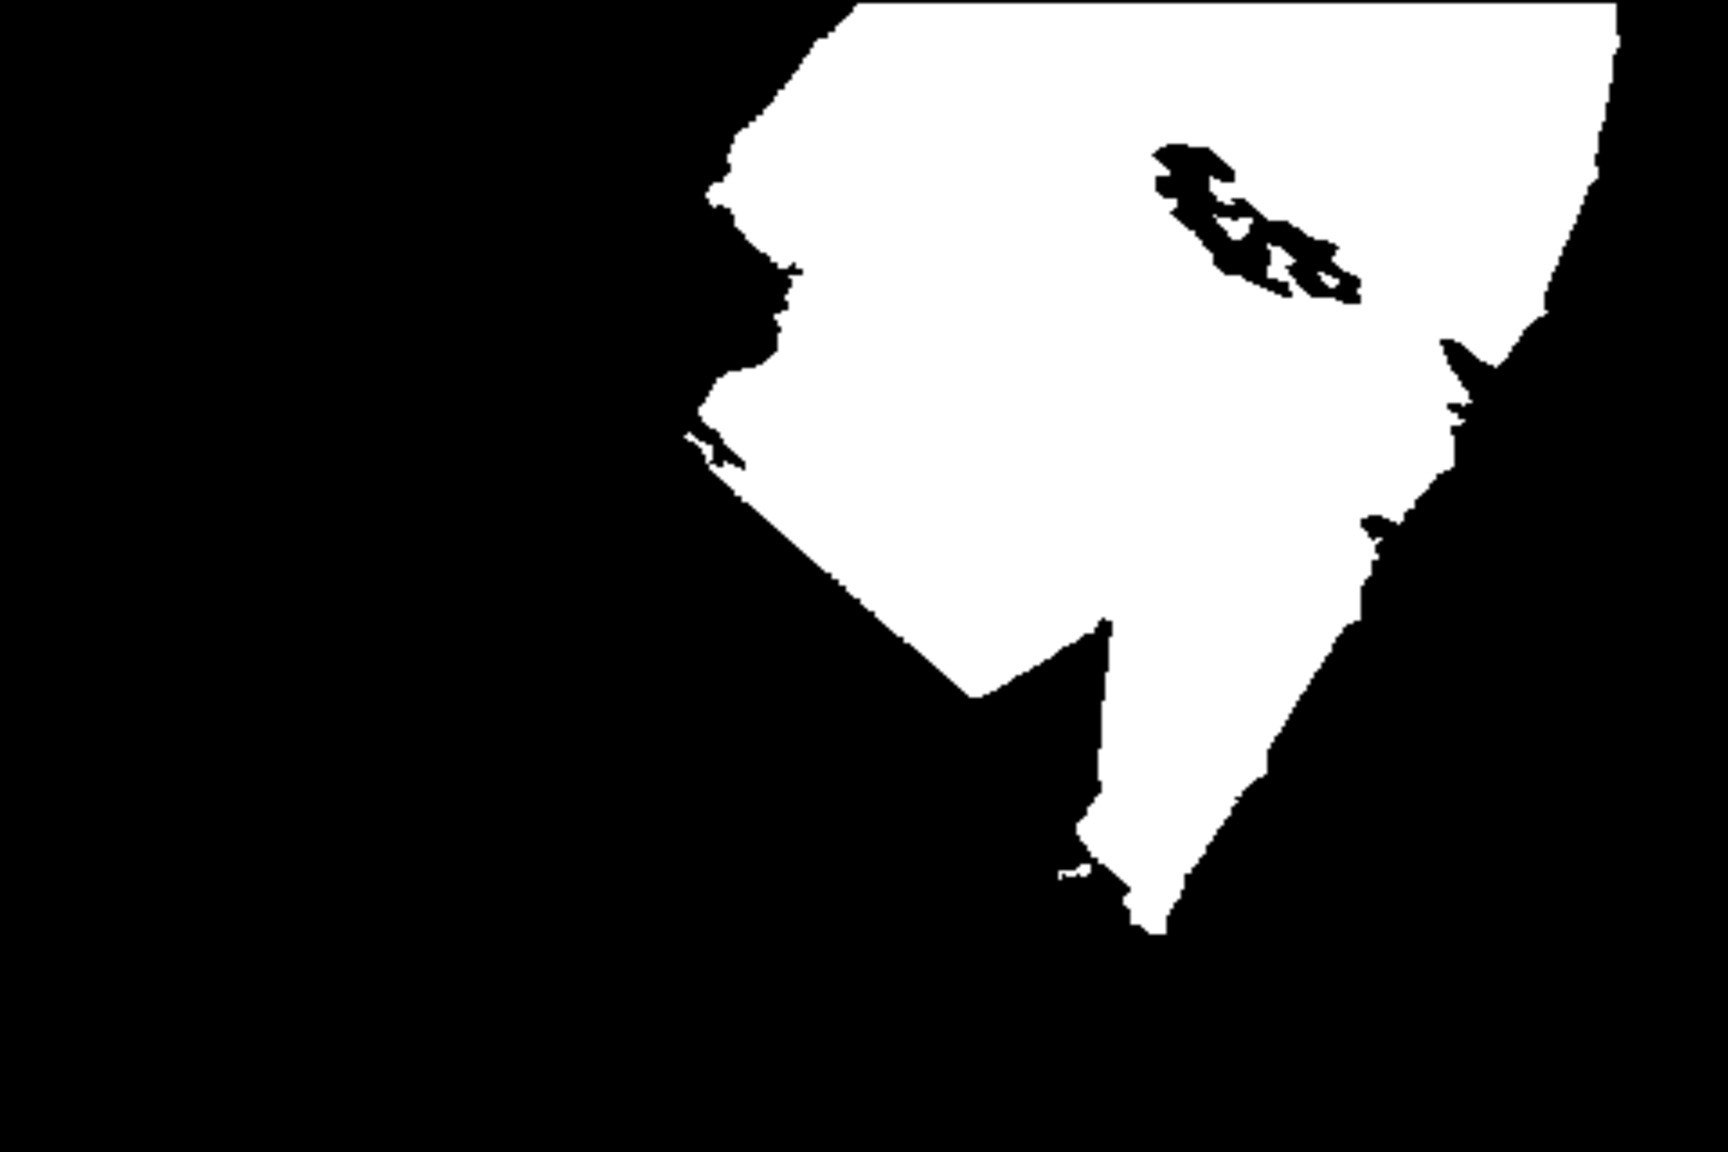
\includegraphics[width=40mm]{FIGS/SkyMask/im_px_005.JPG}
			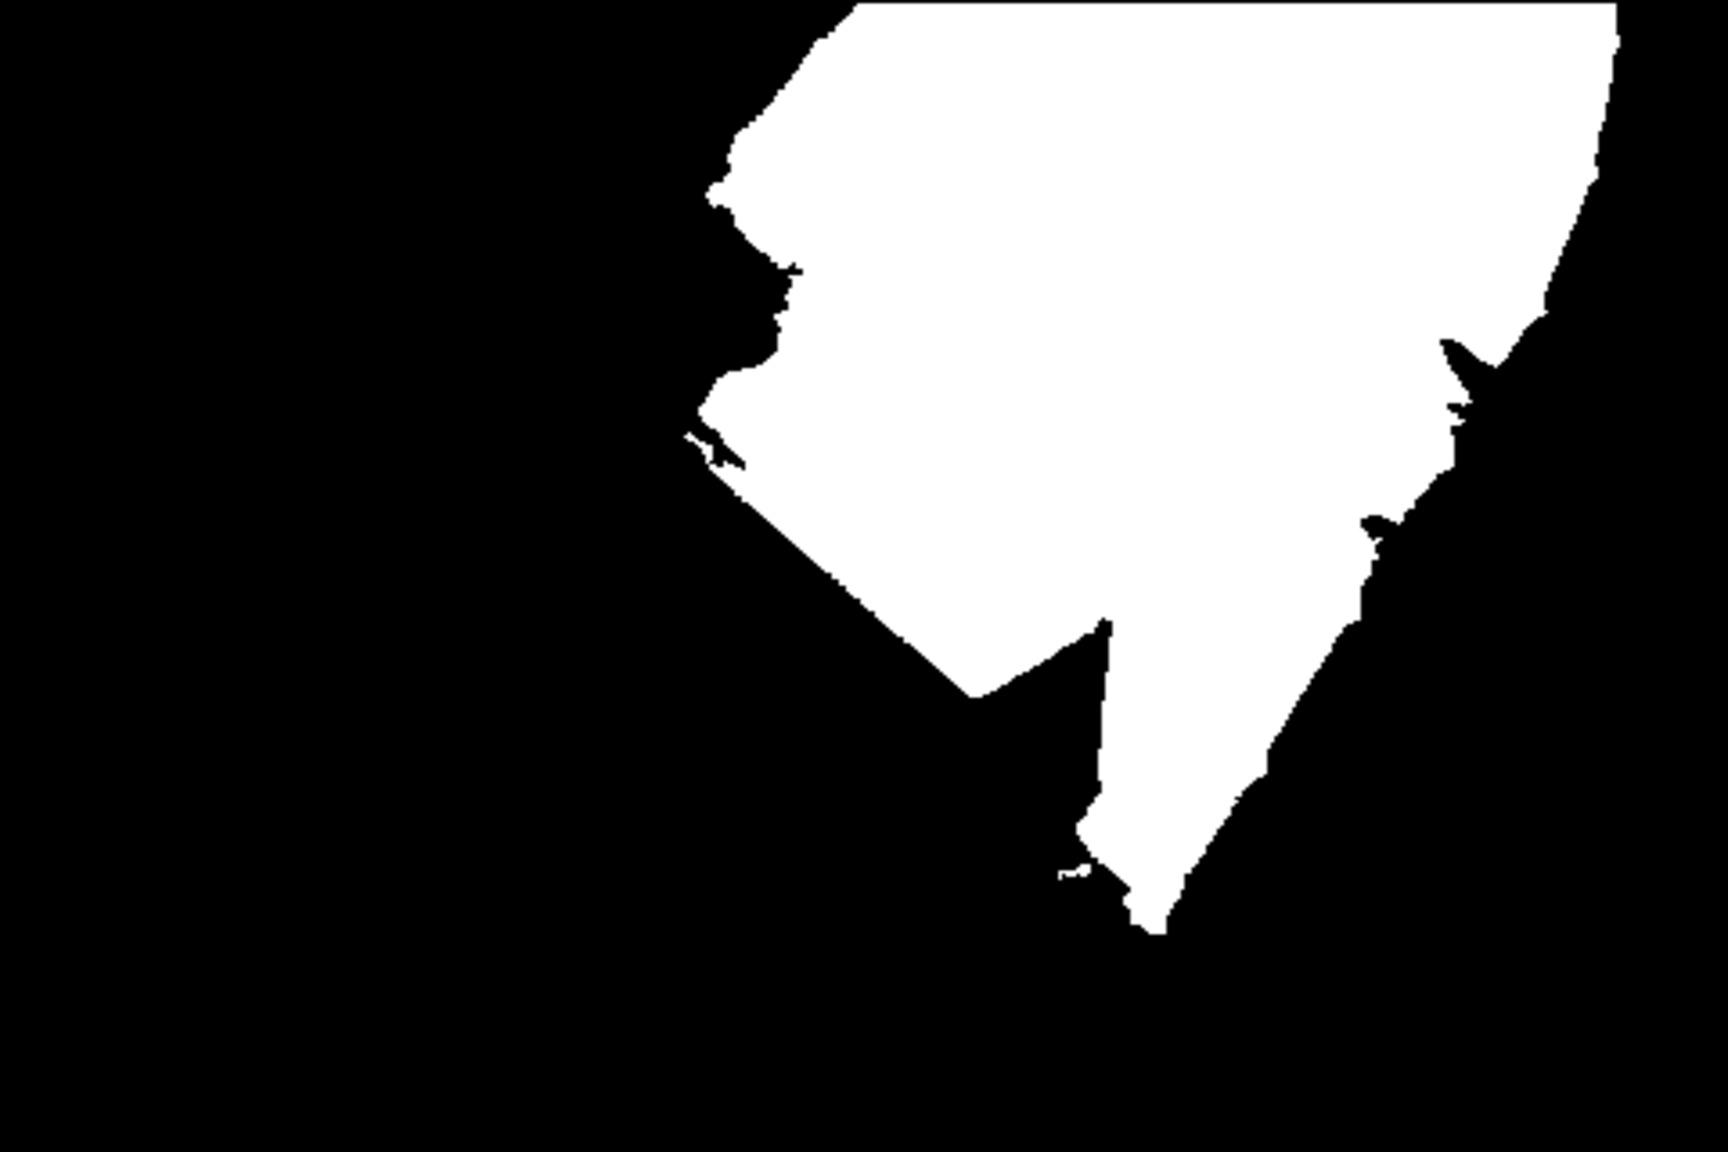
\includegraphics[width=40mm]{FIGS/SkyMask/im_px_01.JPG}
			\caption{Filtering artifacts for a typical image relative size of (from left to right) 0, 0.05 and 0.1.}
		\end{center}	
	\end{figure}

	In general, it is recommened not to be too conservative with this parameter, since non-sky connex components (birds, planes...) are typically not often seen in photogrammetric images. Note that components adjacent to image borders are not considered as individual connex components, and will never be filtered. \newline
	
\end{itemize}




%--------------------------%
\subsection{Homography for tie points}
\vspace{0.5cm}

\noindent In this section we describe how to estimate and use homographic image rectification for tie points search and matching. This tool has been developped for vehicule linear aquisition on highways, where very few tie points may be collected outside the road. In this context, homographic image rectification may assist tie points matching in order to get a more uniform collection of tie points. \newline

\noindent Here, we will consider \textit{Saint-Martin Street} datset, and we will use only images where the road can be clearly seen. \newline

\noindent We start by an approximate orientation of images. This is done classically with the following Micmac instructions : \newline

\begin{verbatim}
mm3d Tapioca All "IMGP41(2[3-9]|3[0-8]).JPG" 1200
mm3d Tapas FishEyeEqui "IMGP41(2[3-9]|3[0-8]).JPG"
\end{verbatim}

\noindent The homographic process is organized in three main commands : \newline
\begin{itemize}
	\item \texttt{EstimHomol} : estimates homographic transformation parameters from a set of ground control points collected on the surface on which we want to rectily images. These points may be digitized with \texttt{SaisieAppuisInit}. In general, this step is done only once for a given sensor (for example, in case of Stereopolis LadyBug camera, it must be done once for each of the 5 horizontal cameras).  \newline 	
	\item \texttt{ApplyHomol} : performs transformation of images with the parameters computed by \texttt{EstimHomol}. Rectified images are stored in a specific folder, where a classical \texttt{Tapioca} process may be launched to compute tie points.   \newline 
	\item \texttt{InvHomolHomog} : performs reverse transformation to project tie points computed on rectified images into the original orientation. Output tie points may then be used in addition to (\texttt{MergeHomol}) original tie points.   \newline 
\end{itemize}

\noindent We use the orientation computed by \texttt{Tapioca} to digitize GCPs on images. A minimal number of 4 points (visible in at least two images) is necessary to compute homographic parameters. However, for more safety, it is suggested to collect at least 5 or 6 points. Note that the spatial extent of these points will be the reference to define the actual area where homography is computed (this means that when no margin is input into \texttt{ApplyHomol}, rectified images will be strictly bounded to the bounding box defined by GCPs used to estimate the homography parameters). \newline

\noindent We use SaisieAppuisInit to collect 6 points on the road, visible on 4 different images. 3D coordinates of points are computed by pseudo-intersection. \newline

\begin{verbatim}
mm3d SaisieAppuisInit "IMGP412[3-9].JPG" Ori-FishEyeEqui/ toto mesure.xml
\end{verbatim}

\begin{figure}[!h]
	\begin{center}
		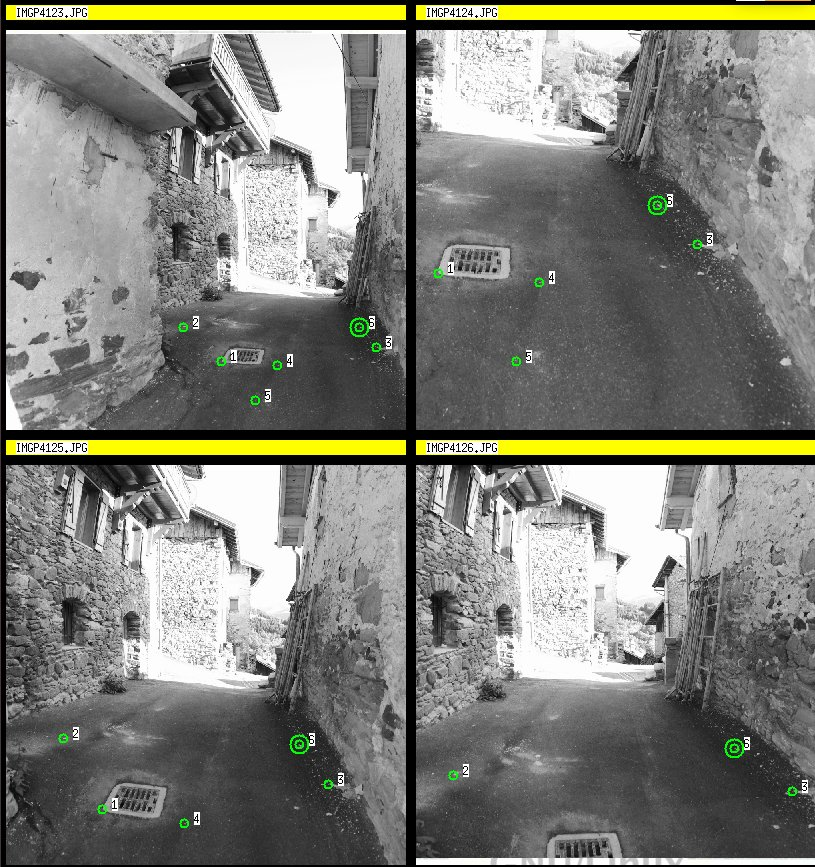
\includegraphics[width=60mm]{FIGS/StreetSainMartin/saisieAppuisHomol.jpg}
		\caption{Collection of 6 points on Saint-Martin Street dataset}
	\end{center}	
\end{figure}

\noindent Output 2D and 3D coordinates of digitized points are collected in \texttt{mesure-S2D.xml} and \texttt{mesure-S3D.xml} respectively. These two files may be used to compute parameters of the homographic transformation :
\newline

$$\left(
\begin{array}{c}
X\\
Y\\
\end{array}
\right)_{road} \rightarrow \mathcal{H}\left(\begin{array}{c}
X\\
Y\\
\end{array}\right)_{road} = \left(\begin{array}{c}
X\\
Y\\
\end{array}\right)_{img}$$ \newline

\noindent where $(.)_{img}$ denotes image coordinates of the collected points (coordinates are defined in one reference image, which is choosen automatically, by default, as the image containing most points). On the other hand, $(.)_{road}$, denotes ground coordinates of GCPs, measured in a reference plane frame contained in the road (technically it is computed as a least squares regression plane of all points). The homographic transformation $\mathcal{H}$ seeks to put in relations these two quantities. It is a $3 \times 3$ real matrix, with 8 degrees of freedom. \newline

\noindent Note that homographic transformation is valid only if points are coplanar (at least to a satisfactory level), and if distorsions are small. When distorsions cannot be neglected, orientation folder needs to be specified to \texttt{EstimHomol} and distorsions will be taken into account as: \newline

$$\left(
\begin{array}{c}
X\\
Y\\
\end{array}
\right)_{road} \rightarrow \mathcal{D} \circ \mathcal{H}\left(\begin{array}{c}
X\\
Y\\
\end{array}\right)_{road} = \left(\begin{array}{c}
X\\
Y\\
\end{array}\right)_{img}$$ \newline

\noindent where $\mathcal{D} : \mathbb{R}^2 \rightarrow \mathbb{R}^2$ stands for the distorsion function, estimated during the intial \texttt{Tapas} internal calibration. \newline

\noindent The 8 unknown parameters of $\mathcal{H}$ are estimated with \texttt{EstimHomol}: \newline

\begin{verbatim}
*****************************
*  Help for Elise Arg main  *
*****************************
Mandatory unnamed args : 
* string :: {Ground 3D points coordinates file}
* string :: {Image 2D points measurement file}
Named args : 
* [Name=Ori] string :: {Orientation folder}
* [Name=ImRef] string :: {Name of reference image}
* [Name=Margin] string :: {Ground 3D points margin}
* [Name=CamRot] bool :: {Camera frame rotation}
\end{verbatim}

\noindent Essentially, it takes as input, 3D and 2D coordinates output from \texttt{SaisieAppuisInit} (make sure that initial orientation is accurate enough to compute relatively precise 3D coordinates). \newline

\noindent Orientation folder needs to be provided in \texttt{Ori}, when distorsions are not negligible, or when \texttt{CamRot} is set to 1 (which aligns rectified images to the sensor orientation). \newline

\noindent \texttt{ImRef} option is used when we want to force the selection of a particular image as reference frame for image 2D coordinates in homographic transformation. Note that all images (in the current or future datasets) that have the same relative orientation with respect to the road, will share the same homographic parameters. Then \texttt{ImRef} option may be used if we want to force the selection of a very representative image, even if in this image does not contain a maximal number of points (provided that it contains at least 4 points). \newline

\noindent Eventually \texttt{Margin} option enables to set the area used for the homography computation. For instance, a margin set to the value 0.5, means that the area visible in rectified images will be 50\% larger than the actual bounding box of points used for the parameters computation. In some case, it is possible that negative values may be accepted as input (but with no garantee), meaning that, for example, a margin set to -0.5 means that tge visible area is twice as small as the original bounding box. \newline

\begin{verbatim}
mm3d EstimHomog mesure-S3D.xml mesure-S2D.xml Ori=FishEyeEqui CamRot=1 Margin=0.5
\end{verbatim}

\noindent The program return the following console outut: \newline

\begin{verbatim}
-----------------------------------------------------------------------
HOMOGRAPHIE ESTIMATION                         
-----------------------------------------------------------------------
Number of images in measurement file [mesure-S2D.xml]: 7
IMGP4123.JPG: 6 pts
IMGP4124.JPG: 6 pts
IMGP4125.JPG: 5 pts
SELECTED IMAGE: IMGP4123.JPG  (6 pts)
-----------------------------------------------------------------------
Number of 3D ground points in [mesure-S3D.xml]: 6
...
-----------------------------------------------------------------------
Distorsion correction from orientation: [FishEyeEqui]
-----------------------------------------------------------------------
Rotation in camera frame: IMGP4123.JPG
-----------------------------------------------------------------------
Point planarization
RESIDUAL POINT 1   0.069
RESIDUAL POINT 2   0.082
RESIDUAL POINT 3   0.243
RESIDUAL POINT 4   0.013
RESIDUAL POINT 5   0.052
RESIDUAL POINT 6   0.183     RMSE = 0.133 GROUND UNITS
-----------------------------------------------------------------------
Corrected ground points: 
...
-----------------------------------------------------------------------
Bounding box:
xmin: -16.75  xmax:  10.09
ymin:  23.99  ymax:  45.66
-----------------------------------------------------------------------
Solving least squares
RESIDUAL POINT 1   2.571 PX
RESIDUAL POINT 2   1.425 PX
RESIDUAL POINT 3   1.564 PX
RESIDUAL POINT 4   3.085 PX
RESIDUAL POINT 5   3.110 PX
RESIDUAL POINT 6   1.600 PX     RMSE = 2.34 PX
-----------------------------------------------------------------------
H =   -105.537   -124.917    847.206
       -14.651    -82.052   -387.203
        -0.018     -0.145      1.000
-----------------------------------------------------------------------
Homography parameters written in [homog.xml] file
-----------------------------------------------------------------------
\end{verbatim}

\noindent Among important informations, we have: \newline

\begin{itemize}
	\item \textbf{Input statistics:} the number of images in 2D measurement file, the number of 3D points and the numbers of points per image. The selected reference image (IMGP4123.JPG), \textit{i.e.} by default one that maximizes the number of visible points, is also displayed. \newline
	\item \textbf{Point planirization statistics:} the plane regression residual for each 3D point (in ground units). Here we have 13 cm, which means that input points are relatively coplanar. \newline
	\item \textbf{Bounding box:} the 3D coordinates (in input orientation units) of the definition domain of the homography. \newline
	\item \textbf{Homography statistics:} least squares residual (in pixels) for each 3D point. Here we have a root mean square error of 2.34 pixels, with a maximal value of about 3 pixels. \newline
	\item \textbf{Homography parameters:} given in the form of a $3 \times 3$ matrix, with 8 DOF. \newline
\end{itemize}

\noindent Homography parameters (along with its definition domain) are saved in \texttt{homog.xml}. This file can then be input into \texttt{ApplyHomog} to transform a batch of images: \newline

\begin{verbatim}
*****************************
*  Help for Elise Arg main  *
*****************************
Mandatory unnamed args : 
* string :: {Images pattern}
* string :: {Homography parameters file}
Named args : 
* [Name=Out] string :: {Output folder}
* [Name=Calib] string :: {Calibration xml file}
* [Name=ImRes] string :: {Output resolution of images}
* [Name=Interp] string :: {Interpolation method (ppv/bilin)}
\end{verbatim}


\noindent By default, rectified images are saved in \texttt{Homog} directory. Default resolution is 2000 px (in the largest direction), and default interpolation method is bilinear interpolation. When distorsion $\mathcal{D}$ has been taken into account for homography computation, it myst be provided in input (through its xml file in orienattion directory). \newline

\begin{verbatim}
mm3d ApplyHomog "IMG.*.JPG" homog.xml Calib=Ori-FishEyeEqui/AutoCal_Foc-10000_Cam-PENTAX_K5.xml
\end{verbatim}

\noindent As a result, all images are rectified with \texttt{homog.xml} parameters. \newline

\begin{figure}[!h]
	\begin{center}
		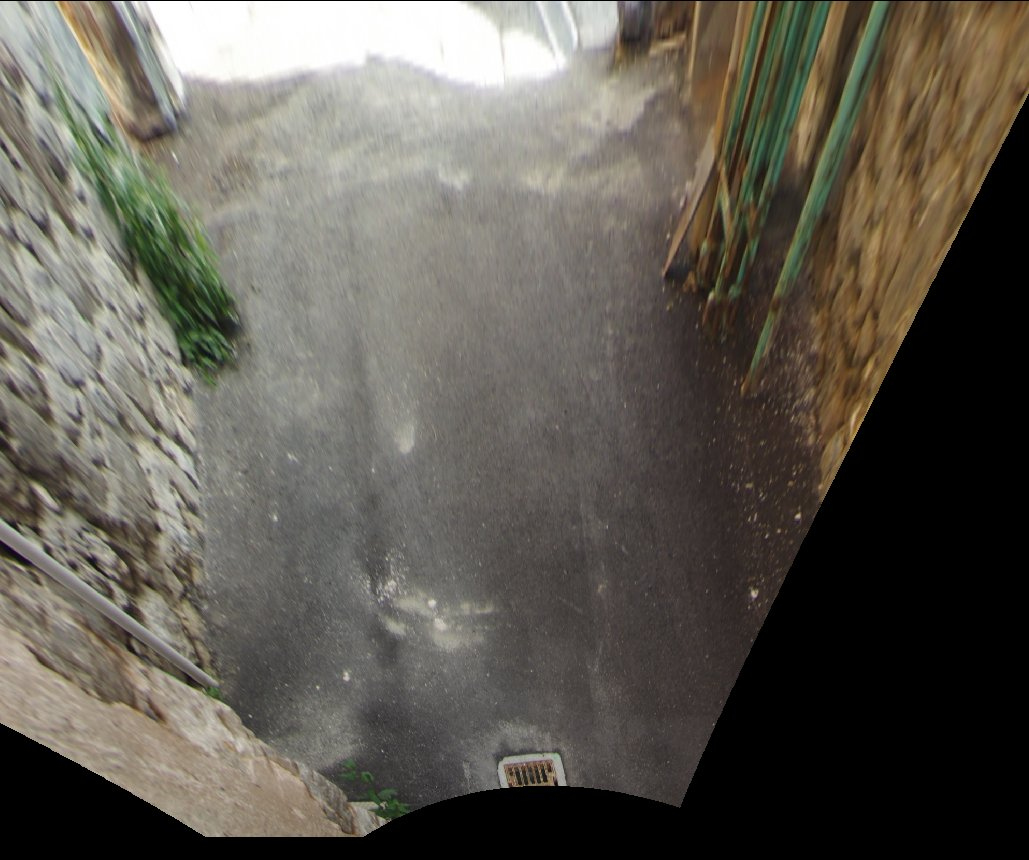
\includegraphics[width=70mm]{FIGS/StreetSainMartin/rectified.jpg}
		\caption{Output of homographic transformation.}
	\end{center}	
\end{figure}

\noindent Then, a classifcal tie point computation may be performed on the rectified images (note that output images are .tif) \newline

\begin{verbatim}
cd Homog/
mm3d Tapioca All "IMGP41(2[3-9]|3[0-8]).tif" 1200
\end{verbatim} 

\begin{figure}[!h]
	\begin{center}
		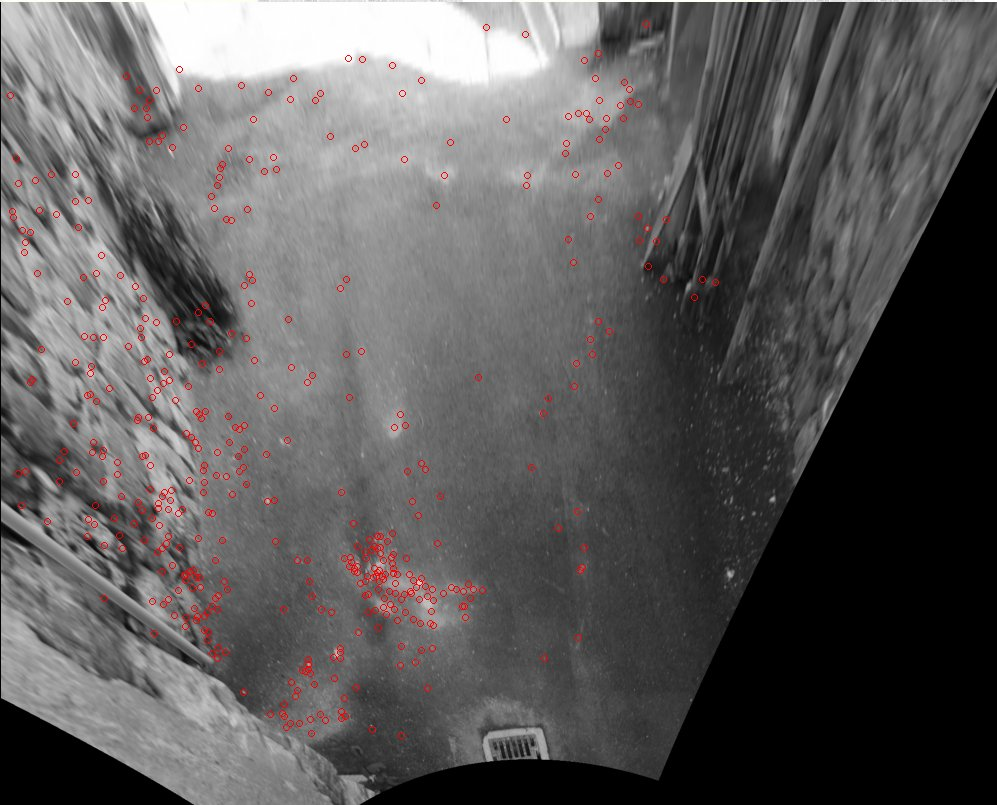
\includegraphics[width=52mm]{FIGS/StreetSainMartin/rect_tie1.jpg}
		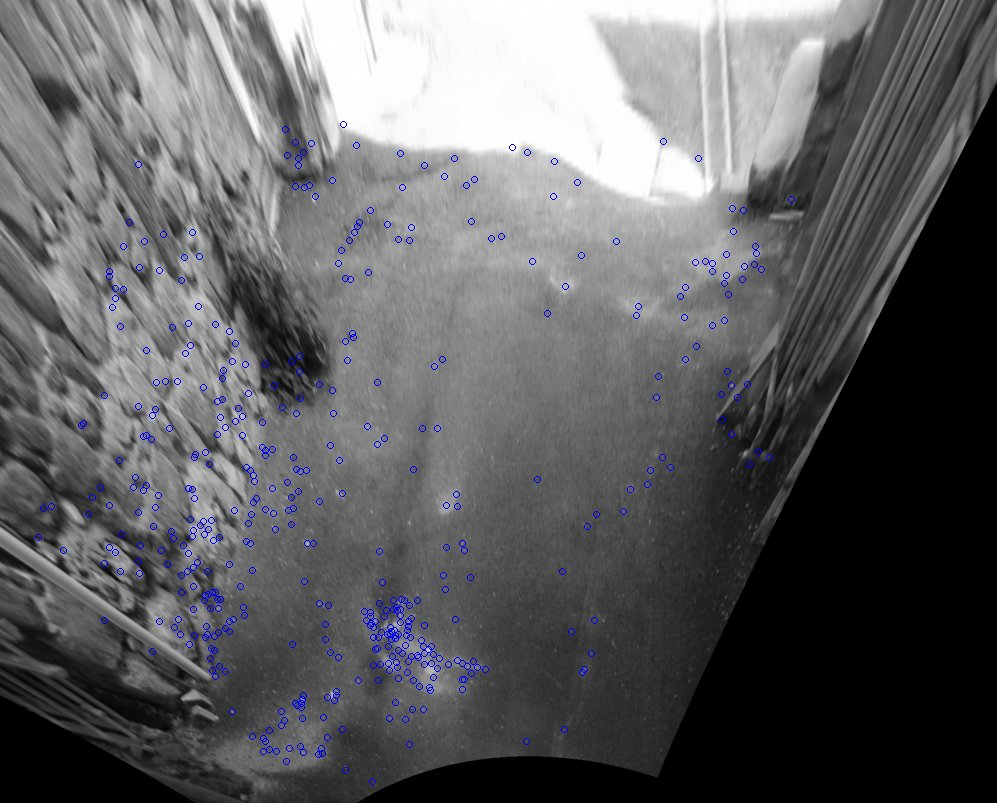
\includegraphics[width=52mm]{FIGS/StreetSainMartin/rect_tie2.jpg}
		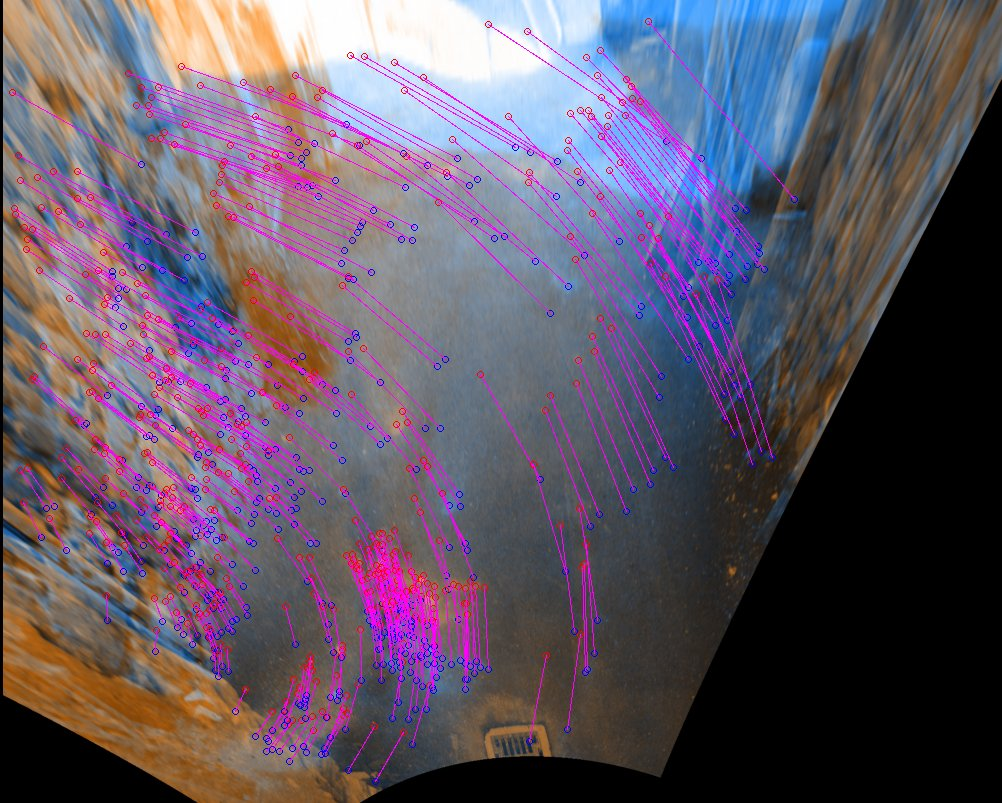
\includegraphics[width=52mm]{FIGS/StreetSainMartin/rect_tie3.jpg}
		\caption{Tie points computation on a pair of rectified images.}
	\end{center}	
\end{figure}

\noindent \texttt{InvHomolHomog} is then executed to transform tie points back to the original orientation. \newline



\begin{verbatim}
*****************************
*  Help for Elise Arg main  *
*****************************
Mandatory unnamed args : 
* string :: {Rectified images pattern}
* string :: {Raw images folder}
* string :: {Homography parameters file}
Named args : 
* [Name=Calib] string :: {Calibration xml file}
* [Name=Out] string :: {Homol output folder}
* [Name=ExpTxtIn] string :: {Input in txt}
* [Name=ExpTxtOut] string :: {Output in txt}
* [Name=Ext] string :: {Target image extension}
\end{verbatim} 
\vspace{0.5cm}

\noindent Here also, if homography has been computed with distorsion $\mathcal{D}$, xml intrinsic calibration file must be provided. Also, target image extension (here \texttt{JPG}) may be specified (in case, like here, original images are not .tif). \newline

\begin{verbatim}
mm3d InvHomolHomog "IMGP41(2[3-9]|3[0-8]).tif" ../ ../homog.xml
Calib=../Ori-FishEyeEqui/AutoCal_Foc-10000_Cam-PENTAX_K5.xml Ext=JPG
\end{verbatim} 


\noindent By default \texttt{HomolInvHomog} folder is created. It can be merged with original tie points folder: \newline

\begin{verbatim}
mv HomolInvHomog ../
cd ../
mm3d MergeHomol Homol.* HomolAll
\end{verbatim} 

\noindent All tie points (original plus collected after rectification) may be visualized: \newline

\begin{verbatim}
mm3d SEL './' IMGP4125.JPG IMGP4126.JPG KH=NB SH=All
\end{verbatim} 

\noindent Also, we can compare individually original and rectified groups: \newline

\begin{verbatim}
mm3d SEL './' IMGP4125.JPG IMGP4126.JPG KH=NB
mm3d SEL './' IMGP4125.JPG IMGP4126.JPG KH=NB SH=InvHomog
\end{verbatim} 

\begin{figure}[!h]
	\begin{center}
		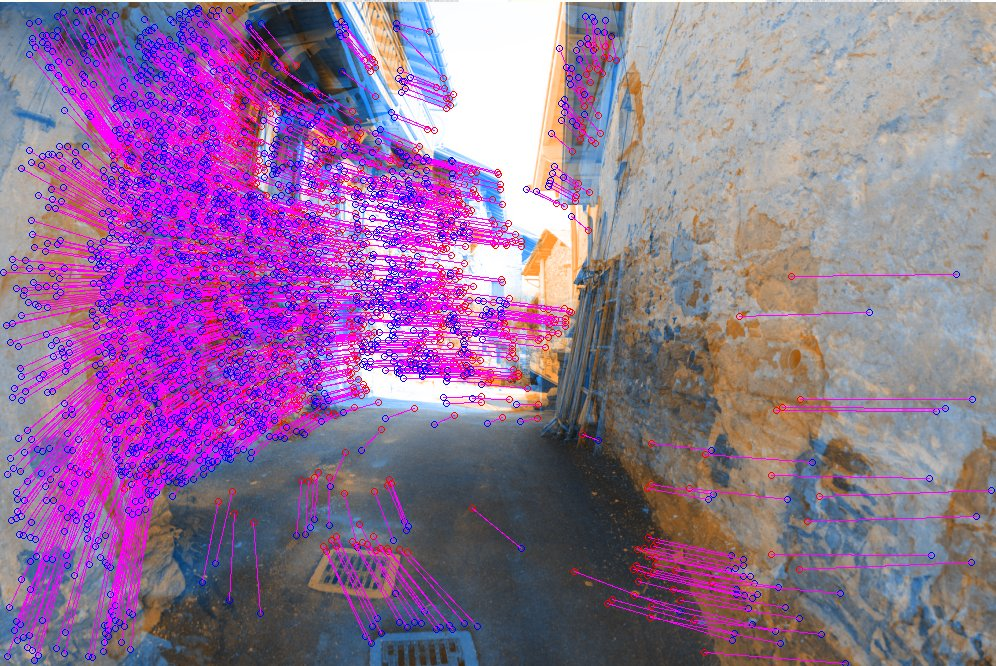
\includegraphics[width=52mm]{FIGS/StreetSainMartin/rect2.jpg}
		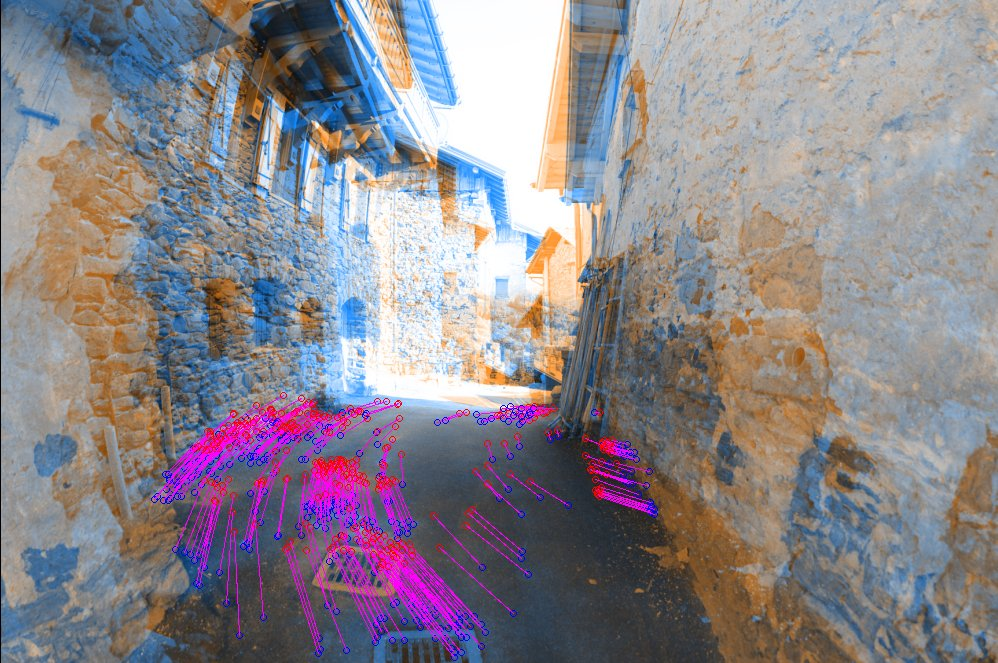
\includegraphics[width=52mm]{FIGS/StreetSainMartin/rect1.jpg}
		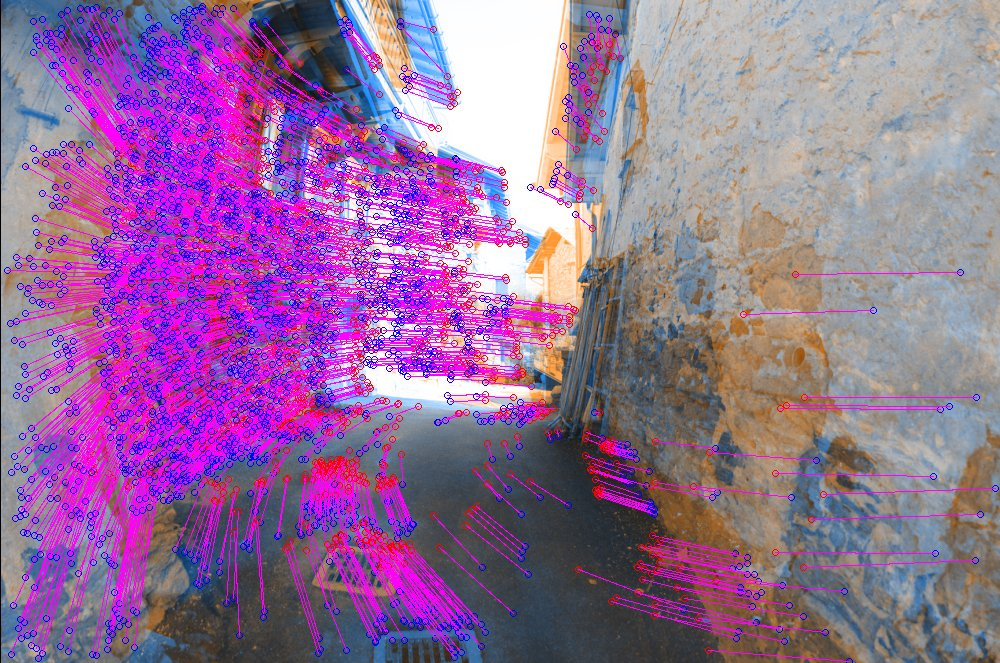
\includegraphics[width=52mm]{FIGS/StreetSainMartin/rect3.jpg}
		\caption{Left: original tie points. Center: complementary tie points computed on rectified images. Right: all tie points merged together.}
	\end{center}	
\end{figure}

\noindent Eventually, we can use \texttt{Schnaps} tool to remove redundant points ang get a more uniform coverage: \newline

\begin{verbatim}
mm3d Schnaps "IMGP41(2[3-9]|3[0-8]).JPG" HomolIn=All HomolOut=AllReduced
mm3d SEL './' IMGP4125.JPG IMGP4126.JPG KH=NB SH=AllReduced
\end{verbatim} 

\begin{figure}[!h]
	\begin{center}
		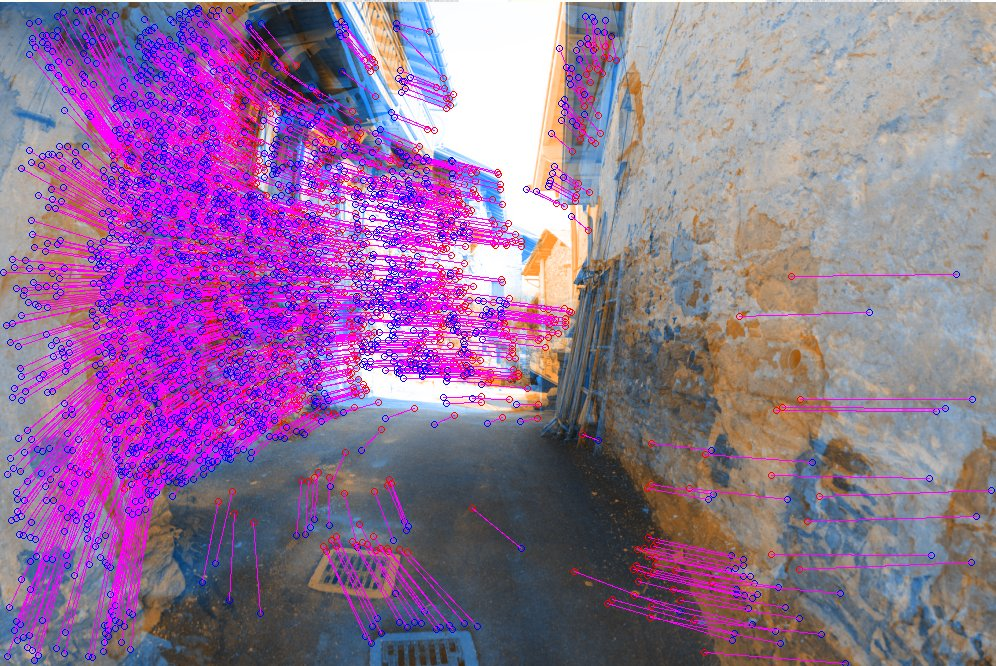
\includegraphics[width=75mm]{FIGS/StreetSainMartin/rect2.jpg}
		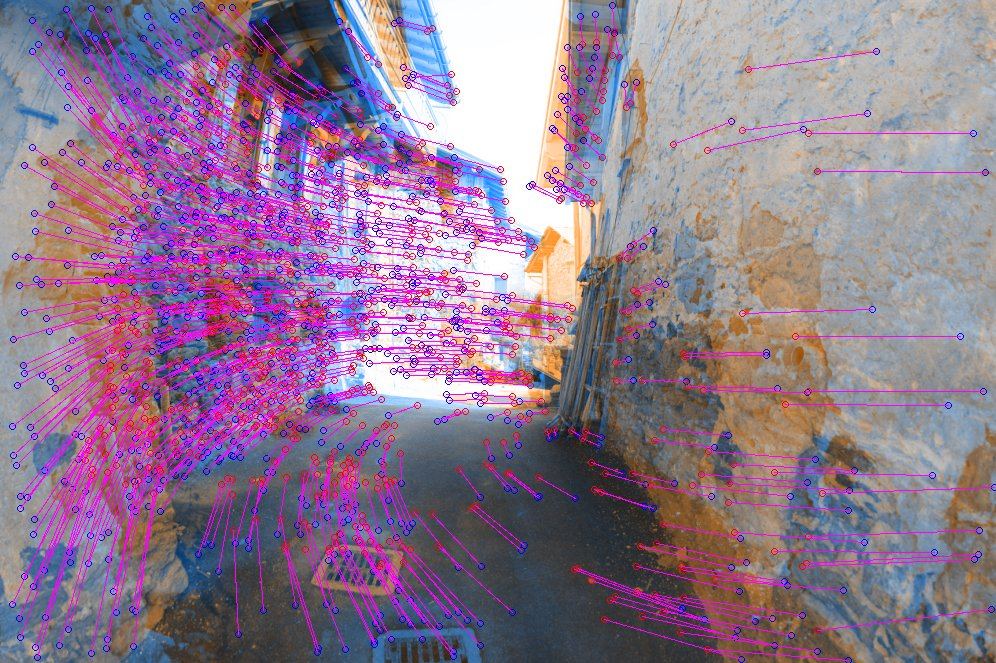
\includegraphics[width=75mm]{FIGS/StreetSainMartin/rect4.jpg}
		\caption{Left: original tie points. Right: all tie points merged and reduced with \texttt{Schnaps}.}
	\end{center}	
\end{figure}
%--------------------------%

\section{Simulation tools}
\subsection{GenerateTP}
The {\tt TestLib GenerateTP} command generates perfectly intersected simulated tie points from a given tie point file (.dat of new format) and a given orientation folder. For now, it is possible to add a gaussian noise or bias from image files.

\begin{verbatim}
mm3d TestLib GenerateTP
*****************************
*  Help for Elise Arg main  *
*****************************
Mandatory unnamed args : 
  * string :: {Image Pattern}
  * string :: {PMul File}
  * string :: {Ori}
Named args : 
  * [Name=Out] string :: {Output name of generated tie points, Def=simulated}
  * [Name=Seed] INT :: {Seed for generating random noise}
  * [Name=NoiseGaussian] vector<double> :: {[meanX,stdX,meanY,stdY]}
  * [Name=ImNX] string :: {image containing noise on X-axis}
  * [Name=ImNY] string :: {image containing noise on Y-axis}
  * [Name=TP3D] string :: {Output 3D positions of tie points without distortion.}

\end{verbatim}

Example :
\begin{verbatim}
mm3d TestLib GenerateTP im.*.tif Homol/PMulAll.dat Ori-Cmp/ Out=test NoiseGaussian=[10,5,10,5]
mm3d TestLib GenerateTP im.*.tif Homol/PMulAll.dat Ori-Cmp/ Out=test ImNX=biasX.tif ImNY=biasY.tif
\end{verbatim}
C++ takes a seed for generating a random noise, the seed is saved in file Seed.txt. If one wants to regenerate a certain random noise, the seed should be given.


\subsection{GenerateMAF}
The {\tt TestLib GenerateMAF} command generates perfect image measurements from a given GCP file and a given orientation folder. It is possible to add bias from images files.

\begin{verbatim}
mm3d TestLib GenerateMAF
*****************************
*  Help for Elise Arg main  *
*****************************
Mandatory unnamed args : 
  * string :: {Image pattern}
  * string :: {Ori}
  * string :: {File containning GCP coordinates}
Named args : 
  * [Name=Out] string :: {Output name of the generated MAF file, Def=Gen_MAF_Ori.xml}
  * [Name=ImNX] string :: {image containing noise on X-axis}
  * [Name=ImNY] string :: {image containing noise on Y-axis}
\end{verbatim}

Example :
\begin{verbatim}
mm3d TestLib GenerateMAF ./ img.*.tif Ori-Cmp/ Gcps_L93h.xml
\end{verbatim}


